\documentclass[a4paper,reqno,]{article}
\usepackage[utf8]{inputenc}
\usepackage[english]{babel}
\usepackage[nosumlimits]{amsmath}
\usepackage{graphicx}
\usepackage{fancyhdr}
\usepackage{hyperref}
\usepackage{caption}
\usepackage{bm}
\usepackage{todonotes}
\usepackage{ctable}
\usepackage[acronym]{glossaries}
\usepackage{subcaption}
\usepackage[left=2cm,right=2cm,top=2.5cm,includeheadfoot]{geometry}
\usepackage{listings}
\usepackage{color, colortbl}
\usepackage{longtable}
\usepackage{booktabs}
\usepackage{tabularx}
\definecolor{Gray}{gray}{0.8}
\renewcommand\lstlistingname{Beispiel}
\usepackage[export]{adjustbox}
\newcommand{\dd}[1]{\mathrm{d}#1}
\usepackage{float}
\usepackage[backend=biber,style=nature,citestyle=authoryear]{biblatex}
\addbibresource{references.bib}
\begin{document}
\begin{titlepage}
\centering
{\scshape University College London \par}
{\scshape faculty of the built environment \par}
\vspace{1cm}
\begin{minipage}[b]{1\textwidth}
\centering
    
\includegraphics[width=0.3\textwidth]{images/ucl_logo.jpg}
\end{minipage}
\newline
\newline
\newline
{\large\bfseries BENVGSC5 Urban Simulation \par}
\vspace{1.5cm}
{\huge\bfseries  Understanding Urban Modelling Methodologies\par}
\vspace{3cm}
{\large Qiqing Huang, 17014982 \par}
\vspace{1cm}
{\large Network: 991 words\par}
{\large ABM: 980 words\par}
{\large Spatial Model: 986 words\par}
\vspace{2cm}
{Centre for Advanced Spatial Analysis \par}
{25$^{\text{th}}$ April, 2018 \par}
\end{titlepage}
\tableofcontents
\newpage
\pagestyle{fancy}
\fancyhf{}
\setlength{\headheight}{25pt}
\headsep=30pt
\rfoot{\thepage}
\renewcommand{\headrulewidth}{0.4pt}
\fancyhead[L]{BENVGSC5 Urban Simulation}

\section{Networks}
\label{sec:net}
\fancyhead[R]{Networks}
\subsection{Introduction}
This article aims at understanding and predicting the potential terrorist attack strategies in case of London underground system using network analysis. Section \ref{ssec:keystations} introduces measures of identifying key stations; Section \ref{ssec:assumptions} derives hypotheses based on different attack aims and numbers of target stations. The final section \ref{ssec:finalresult} compares all the results and get an optimal result.
\\The London underground networks are treated as undirected graphs where nodes represent stations and undirected links represent line segments. In this case, there are 306 nodes and 410 links.
\begin{figure}[h]
\centering
\begin{minipage}[b]{0.49\textwidth}
\centering
    \captionsetup{width=.9\linewidth}
    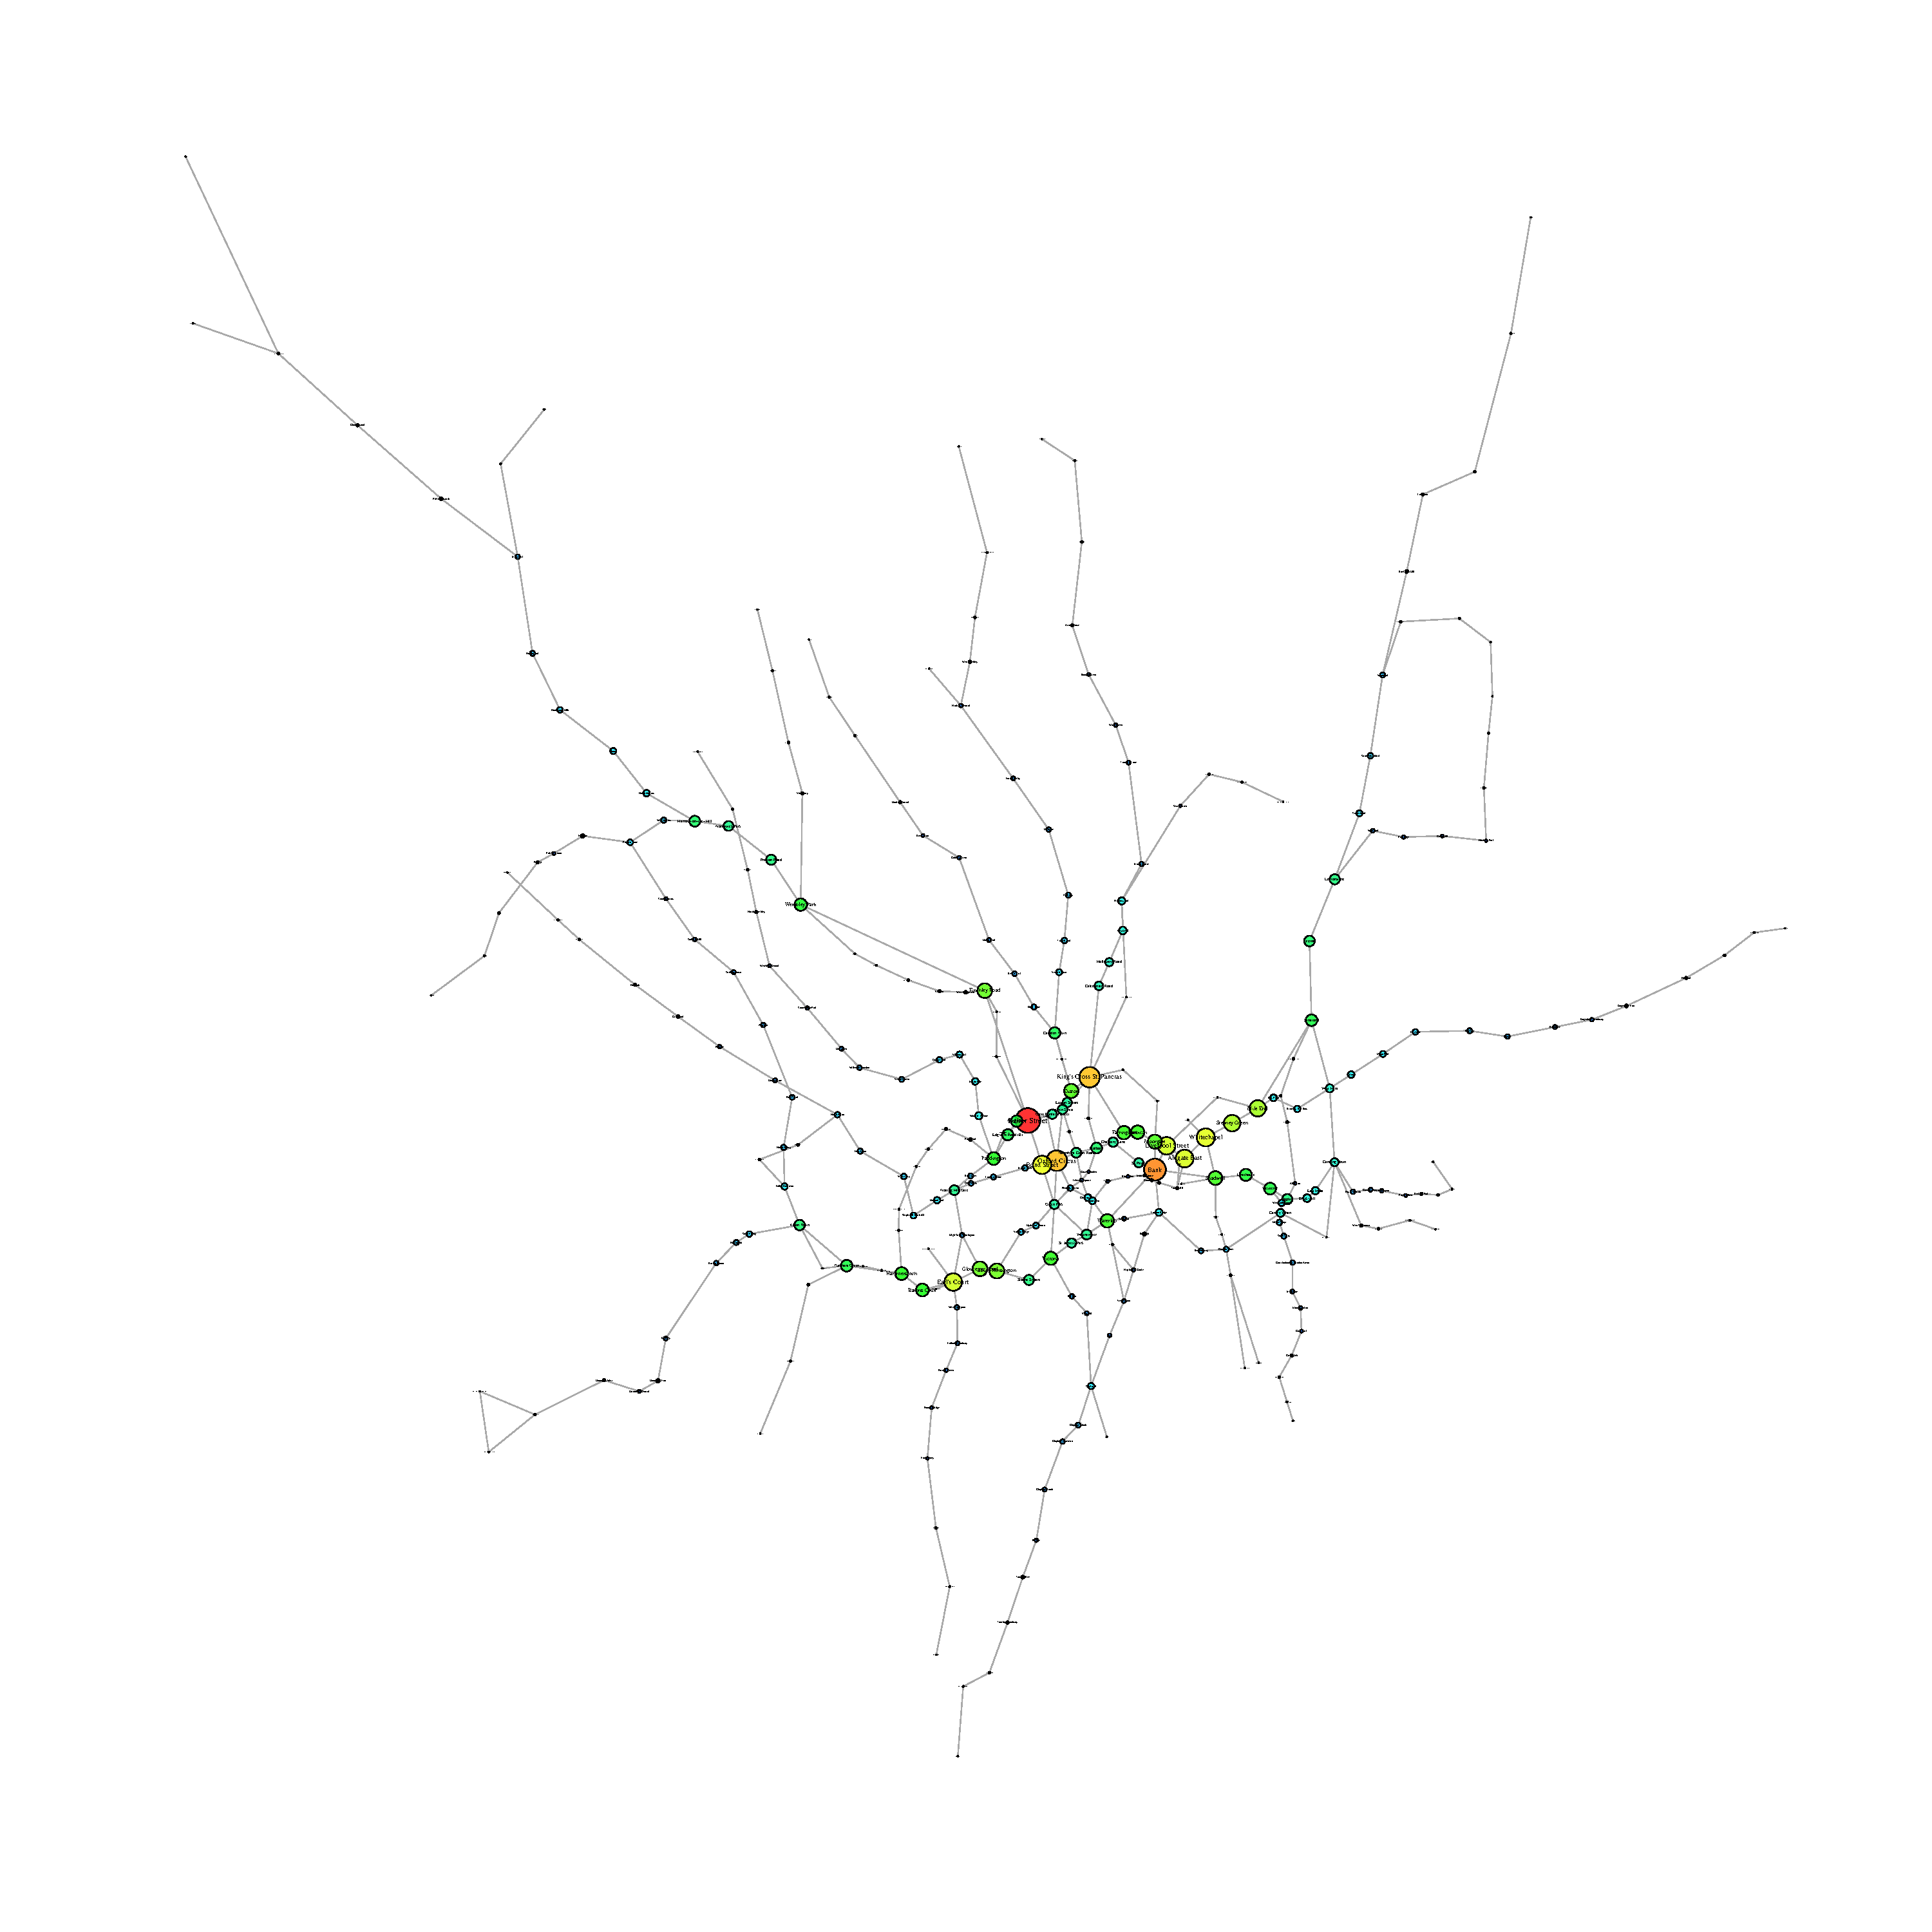
\includegraphics[clip, trim=3cm 3cm 0.25cm 2cm,width=1\textwidth]{images/NW/london_map_w.pdf}
    \caption{The topographical map of the London underground network. Stations of larger betweenness centrality have lager vertex size and more obvious color (Red $>$ Green $>$ Blue). }\label{fig:london_1}
\end{minipage}
\begin{minipage}[b]{0.5\textwidth}
\centering
    \captionsetup{width=.9\linewidth}
    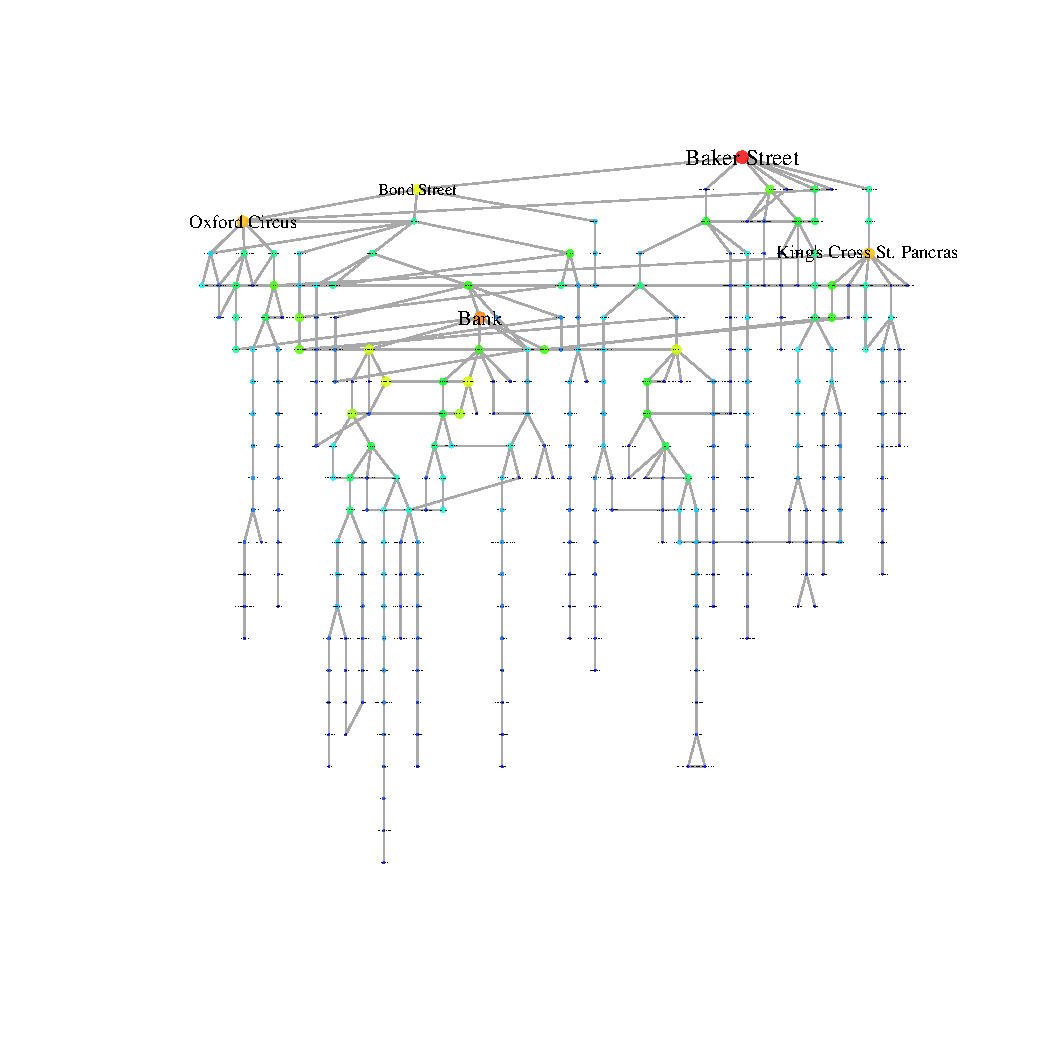
\includegraphics[clip, trim=3cm 3cm 2cm 2cm,width=1\textwidth]{images/NW/london_tree_w.pdf}
    \caption{The tree topology of the London underground network. The top five stations of betweenness centrality are marked by larger label size}\label{fig:london_2}
\end{minipage}
\end{figure} 
\subsection{Identifying Key Stations}
\label{ssec:keystations}
How to identify keyplayers in a network has been widely researched. Among all measures, betweenness centrality is the most popular one as it sums the proportion of shortest paths of all connected pairs that pass by a given node (\cite{freeman1978centrality}). \\Other centrality measures are also checked. The goal of finding targeted attack stations is to find keyplayers that the removing of which would disrupt the network most, which is also known as KPP-NEG problem (\cite{borgatti2006identifying}).
\subsubsection{Centrality Measures of Key Stations}
\begin{enumerate}
\item Degree Centrality
\\Degree centrality measures a node’s direct connectedness with other nodes in a network. Its equation is given as follows (\cite{freeman1978centrality}; \cite{an2016keyplayer}):
\begin{equation}
D_{i} =\sum\limits_{j}{w_{ij}} +\sum\limits_{j}{w_{ji}}
\end{equation}
where $w_{ij}$ means whether it is connected or not from node $i$ to node $j$ and vice versa. 
\item Betweenness Centrality
\\Betweenness centrality usually measures a node’s brokerage power in a network. Its equation is given as follows (\cite{an2016keyplayer}) : 
\begin{equation}
B_{i} = \sum\limits_{jk}\frac{g_{jk}^{i}}{g_{jk}}
\end{equation}
\label{equ:bet}
where $g_{jk}$ is the number of shortest paths between nodes $j$ and $k$, and $g_{jk}^{i}$ is the number of those paths that pass node $i$. When the network consists only isolates which is to say $g_{jk}=0$, the corresponding  betweenness centrality $B_{i}$ equals 1.
\item Eigenvector Centrality
\\Eigenvector centrality measures the importance of the neighbors of a give node. Its equation is given as follows (\cite{an2016keyplayer}):
\begin{equation}
E_{i} = \frac{1}{\lambda}\sum\limits_{j}w_{ij}E_{j}
\end{equation}
\item Fragmentation Centrality
\\Fragmentation Centrality defines a network's fragmentation level based on the reciprocals of distances (after removing a set of nodes from the network) (\cite{borgatti2006identifying}):
\begin{equation}
F = 1-\frac{2\sum\limits_{j,k\neq{i}}{\frac{1}{d_{jk}}}}{d(n-1)(n-2)}
\end{equation}
Where $d_{jk}$ is distance between node $j$ and $k$ after node $i$ is removed.  In the case of $d_{jk}= 0$ , the corresponding fragmentation centrality $F$ is 1.
\end{enumerate}

\subsubsection{Results of Node Centrality}

\begin{table}[H]
 \caption{Top 10 ranked stations based on degree value, unweighted betweenness and unweighted eigenvector centrality value, respectively (All values are normalized)}
 \label{tab:keystation1}
 \begin{center}
 \begin{tabular}{*{6}{c}}
  \toprule
   \multicolumn{2}{c}{Unweighted Degree Centrality} & \multicolumn{2}{c}{Unweighted Betweenness Centrality} & \multicolumn{2}{c}{Unweighted Eigenvector Centrality}\\
  \midrule
   \rowcolor{Gray}\cellcolor{Gray}{King's Cross St. Pancras} & 0.0393 & \cellcolor{Gray}{Waterloo} & 0.3358 & \cellcolor{Gray}{King's Cross St. Pancras} & 1.0000 \\
   \rowcolor{Gray}\cellcolor{Gray}{Baker Street} & 0.0328 & \cellcolor{Gray}{Bank}  & 0.3204 & \cellcolor{Gray}{Farringdon} & 0.8022 \\
    Embankment & 0.0262 & Baker Street & 0.3195 & Euston Square & 0.7593 \\
    Paddington & 0.0262 & Westminster & 0.3026 & Barbican & 0.6474 \\
    Liverpool Street & 0.0262 & Green Park & 0.2980 & Great Portland Street & 0.5595 \\
    Moorgate & 0.0262 & Liverpool Street & 0.2392 & Moorgate & 0.5275 \\
    Earl's Court & 0.0230 & Stratford & 0.2344 & Euston & 0.3968 \\
    Waterloo & 0.0230 & Bond Street & 0.2335 & Baker Street & 0.3896 \\
    Oxford Circus & 0.0197 & Mile End & 0.2237 & Liverpool Street & 0.3428 \\
    Bank  & 0.0197 & Bethnal Green & 0.2145 & Edgware Road (C) & 0.1814 \\
  \bottomrule
 \end{tabular}
 \end{center}
\end{table}
\begin{table}[H]
 \caption{Top 10 ranked stations based on weighted betweenness, weighted fragment centrality value and unweighted fragment centrality value, respectively (All values are normalized)}
 \label{tab:keystation2}
 \begin{center}
 \begin{tabular}{*{6}{c}}
  \toprule
  \multicolumn{2}{c}{Weighted Beteweenness Centrality} & \multicolumn{2}{c}{Weighted Fragment Centrality} & \multicolumn{2}{c}{Unweighted Fragment Centrality} \\
   \midrule
    \rowcolor{Gray}\cellcolor{Gray}{Baker Street} & 0.2846 & \cellcolor{Gray}{Baker Street} & 0.9176 & \cellcolor{Gray}{Euston} & 0.9081 \\
    \rowcolor{Gray}\cellcolor{Gray}{Bank}  & 0.2503 & \cellcolor{Gray}{Euston} & 0.9174 & \cellcolor{Gray}{King's Cross St. Pancras} & 0.9079 \\
    Oxford Circus & 0.2340 & Stratford & 0.9172 & Baker Street & 0.9074 \\
    King's Cross St. Pancras & 0.2328 & King's Cross St. Pancras & 0.9169 & Stratford & 0.9070 \\
    Bond Street & 0.2070 & Camden Town & 0.9166 & Camden Town & 0.9069 \\
    Whitechapel & 0.2049 & Leyton & 0.9159 & Leyton & 0.9057 \\
    Aldgate East & 0.2013 & Leytonstone & 0.9155 & Leytonstone & 0.9052 \\
    Earl's Court & 0.1985 & Finchley Road & 0.9149 & Paddington & 0.9048 \\
    Liverpool Street & 0.1983 & Canning Town & 0.9146 & Finchley Road & 0.9045 \\
    Stepney Green & 0.1866 & Wembley Park & 0.9145 & Canning Town & 0.9042 \\
  \bottomrule
 \end{tabular}
 \end{center}
\end{table}
From table \ref{tab:keystation1} and \ref{tab:keystation2}, it can be seen that  King's Cross St. Pancras has the most direct connections to other stations which indicates it is the most connected traffic hub and the importance is also strengthened by its neighbors as it gets the highest eigenvector value. Besides, its removal leads to fragmentation of the network into two separate parts. As for binary network, Waterloo has the highest betweenness value  and Euston gets the highest fragment value. For distance weighted network, these two highest value holders are all Baker Street station. In the next section, this article will focus on distance weighted situation because it relates more to the real world.
\subsection{Different Assumptions of Attacks}
\label{ssec:assumptions}
As \citeauthor{jordan2008predicting} (\citeyear{jordan2008predicting}) notes, there are different objectives of terrorist attacks including to destroy infrastructure, to hurt normal people, to create panic, etc. Various aims of attacks lead to changing selection of targets. 
\subsubsection{Disrupting the Most Connected Stations}
In terms of destroying the most connected stations, the measurement is based on degree centrality. Therefore, if terrorists choose to damage one station, King's Cross St. Pancras would be targeted. If two stations are selected, King's Cross St. Pancras and Baker Street would be on the list based on the table \ref{tab:keystation1}. The assumption behind this decision is that the more neighbor stations around the target station, the higher potential of more traffic will bring to it in the case that actual traffic data is not available. 
\\In figure \ref{fig: 1_1} and figure \ref{fig: 1_2}, after removing King's Cross St. Pancras, the network is separated into two parts with obvious discrete trend of the change of the structure. The adding of Baker Street does not contribute much in terms of change of whole structure (see figure \ref{fig: 1_2} and \ref{fig: 2_2}). 
\begin{figure}[H]
\centering
\begin{minipage}[b]{0.49\textwidth}
\centering
    \captionsetup{width=.9\linewidth}
    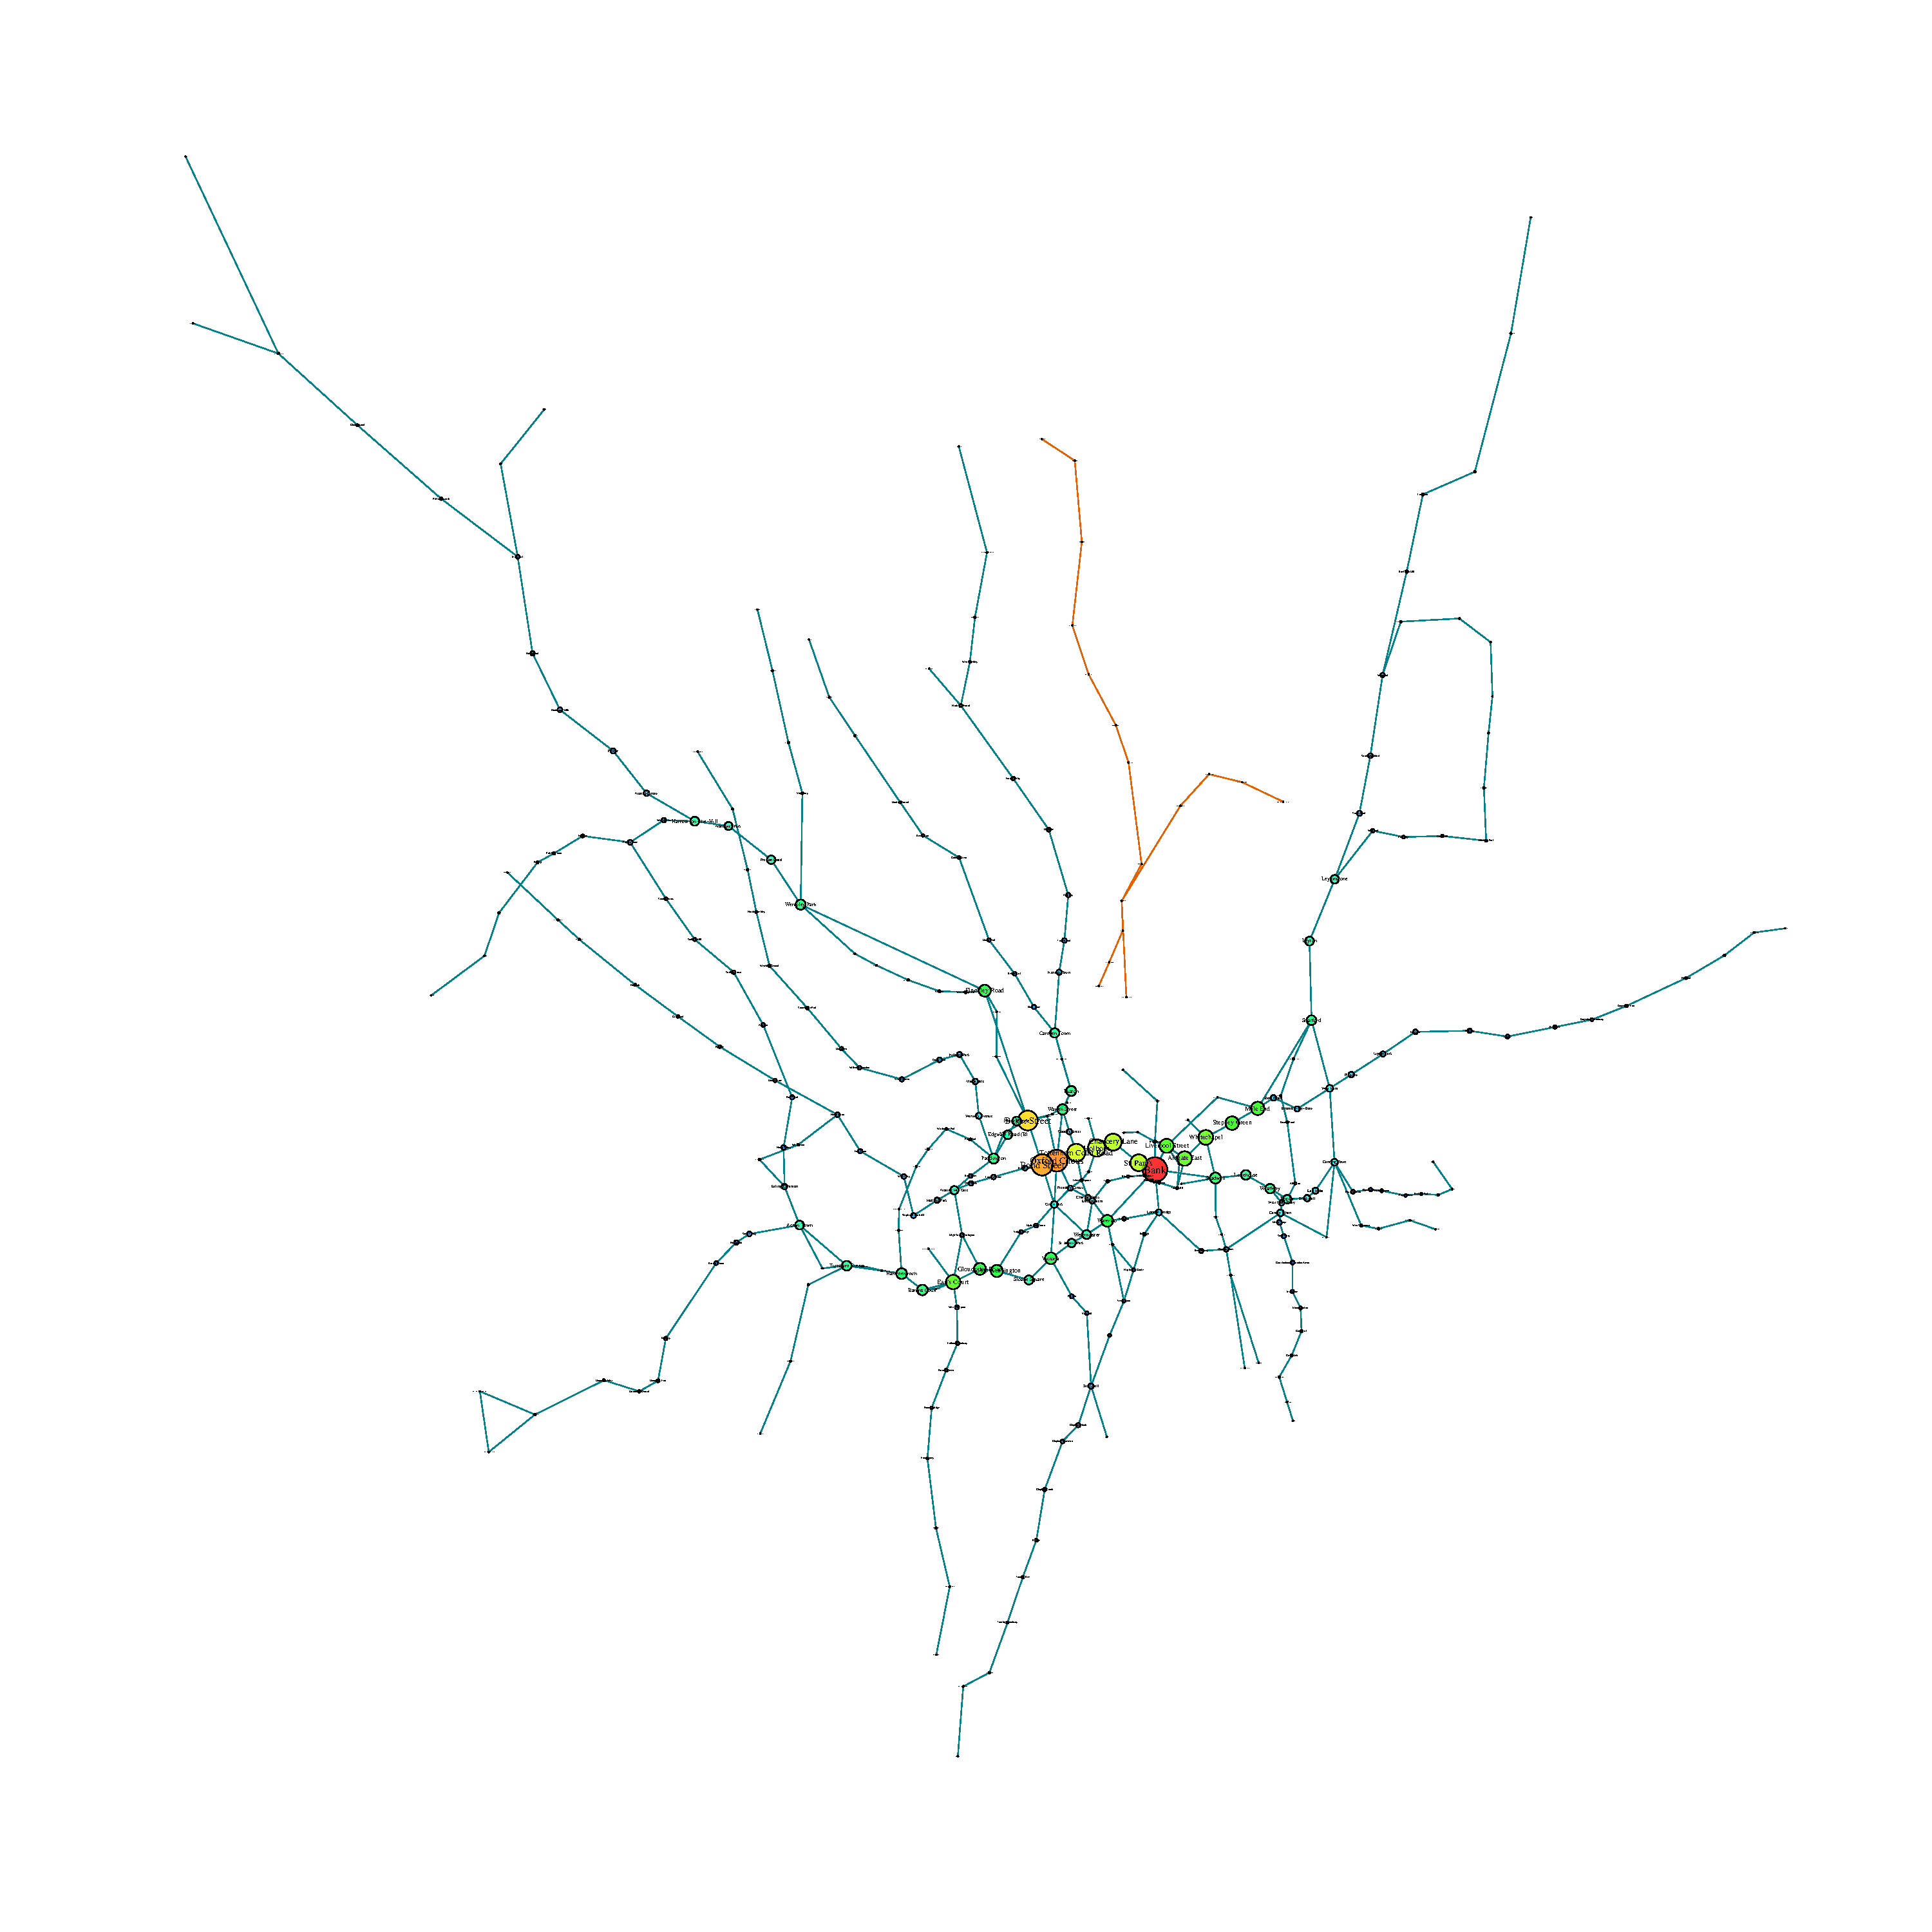
\includegraphics[clip, trim=3cm 3cm 0.25cm 2cm,width=1\textwidth]{images/NW/1_1.pdf}
    \caption{The topographical map of the London underground network after removing King's Cross St. Pancras}\label{fig: 1_1}
\end{minipage}
\begin{minipage}[b]{0.5\textwidth}
\centering
    \captionsetup{width=.9\linewidth}
    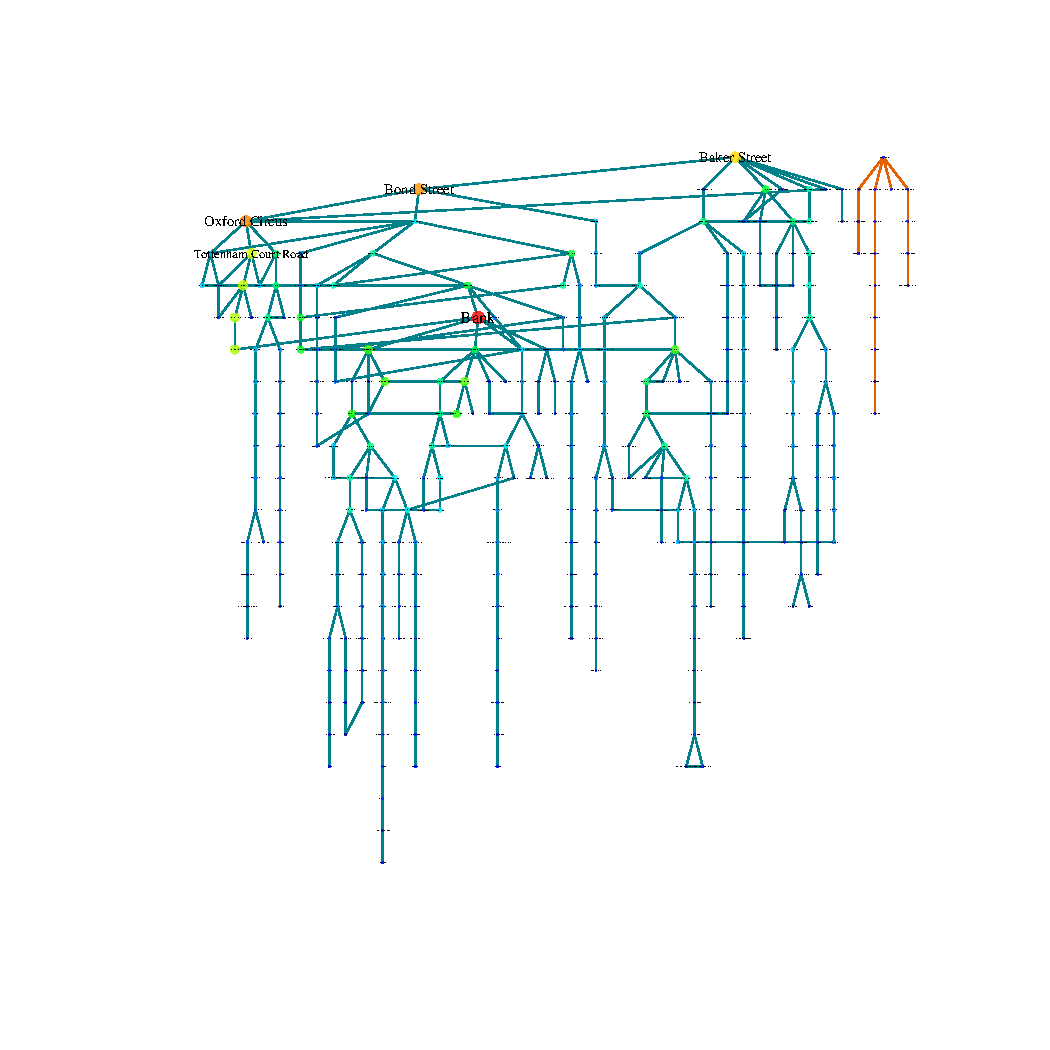
\includegraphics[clip, trim=3cm 3cm 0.25cm 2cm,width=1\textwidth]{images/NW/1_2.pdf}
    \caption{The tree topology of the London underground network after removing King's Cross St. Pancras}\label{fig: 1_2}
\end{minipage}
\end{figure} 
\begin{figure}[h]
\centering
\begin{minipage}[b]{0.49\textwidth}
\centering
    \captionsetup{width=.9\linewidth}
    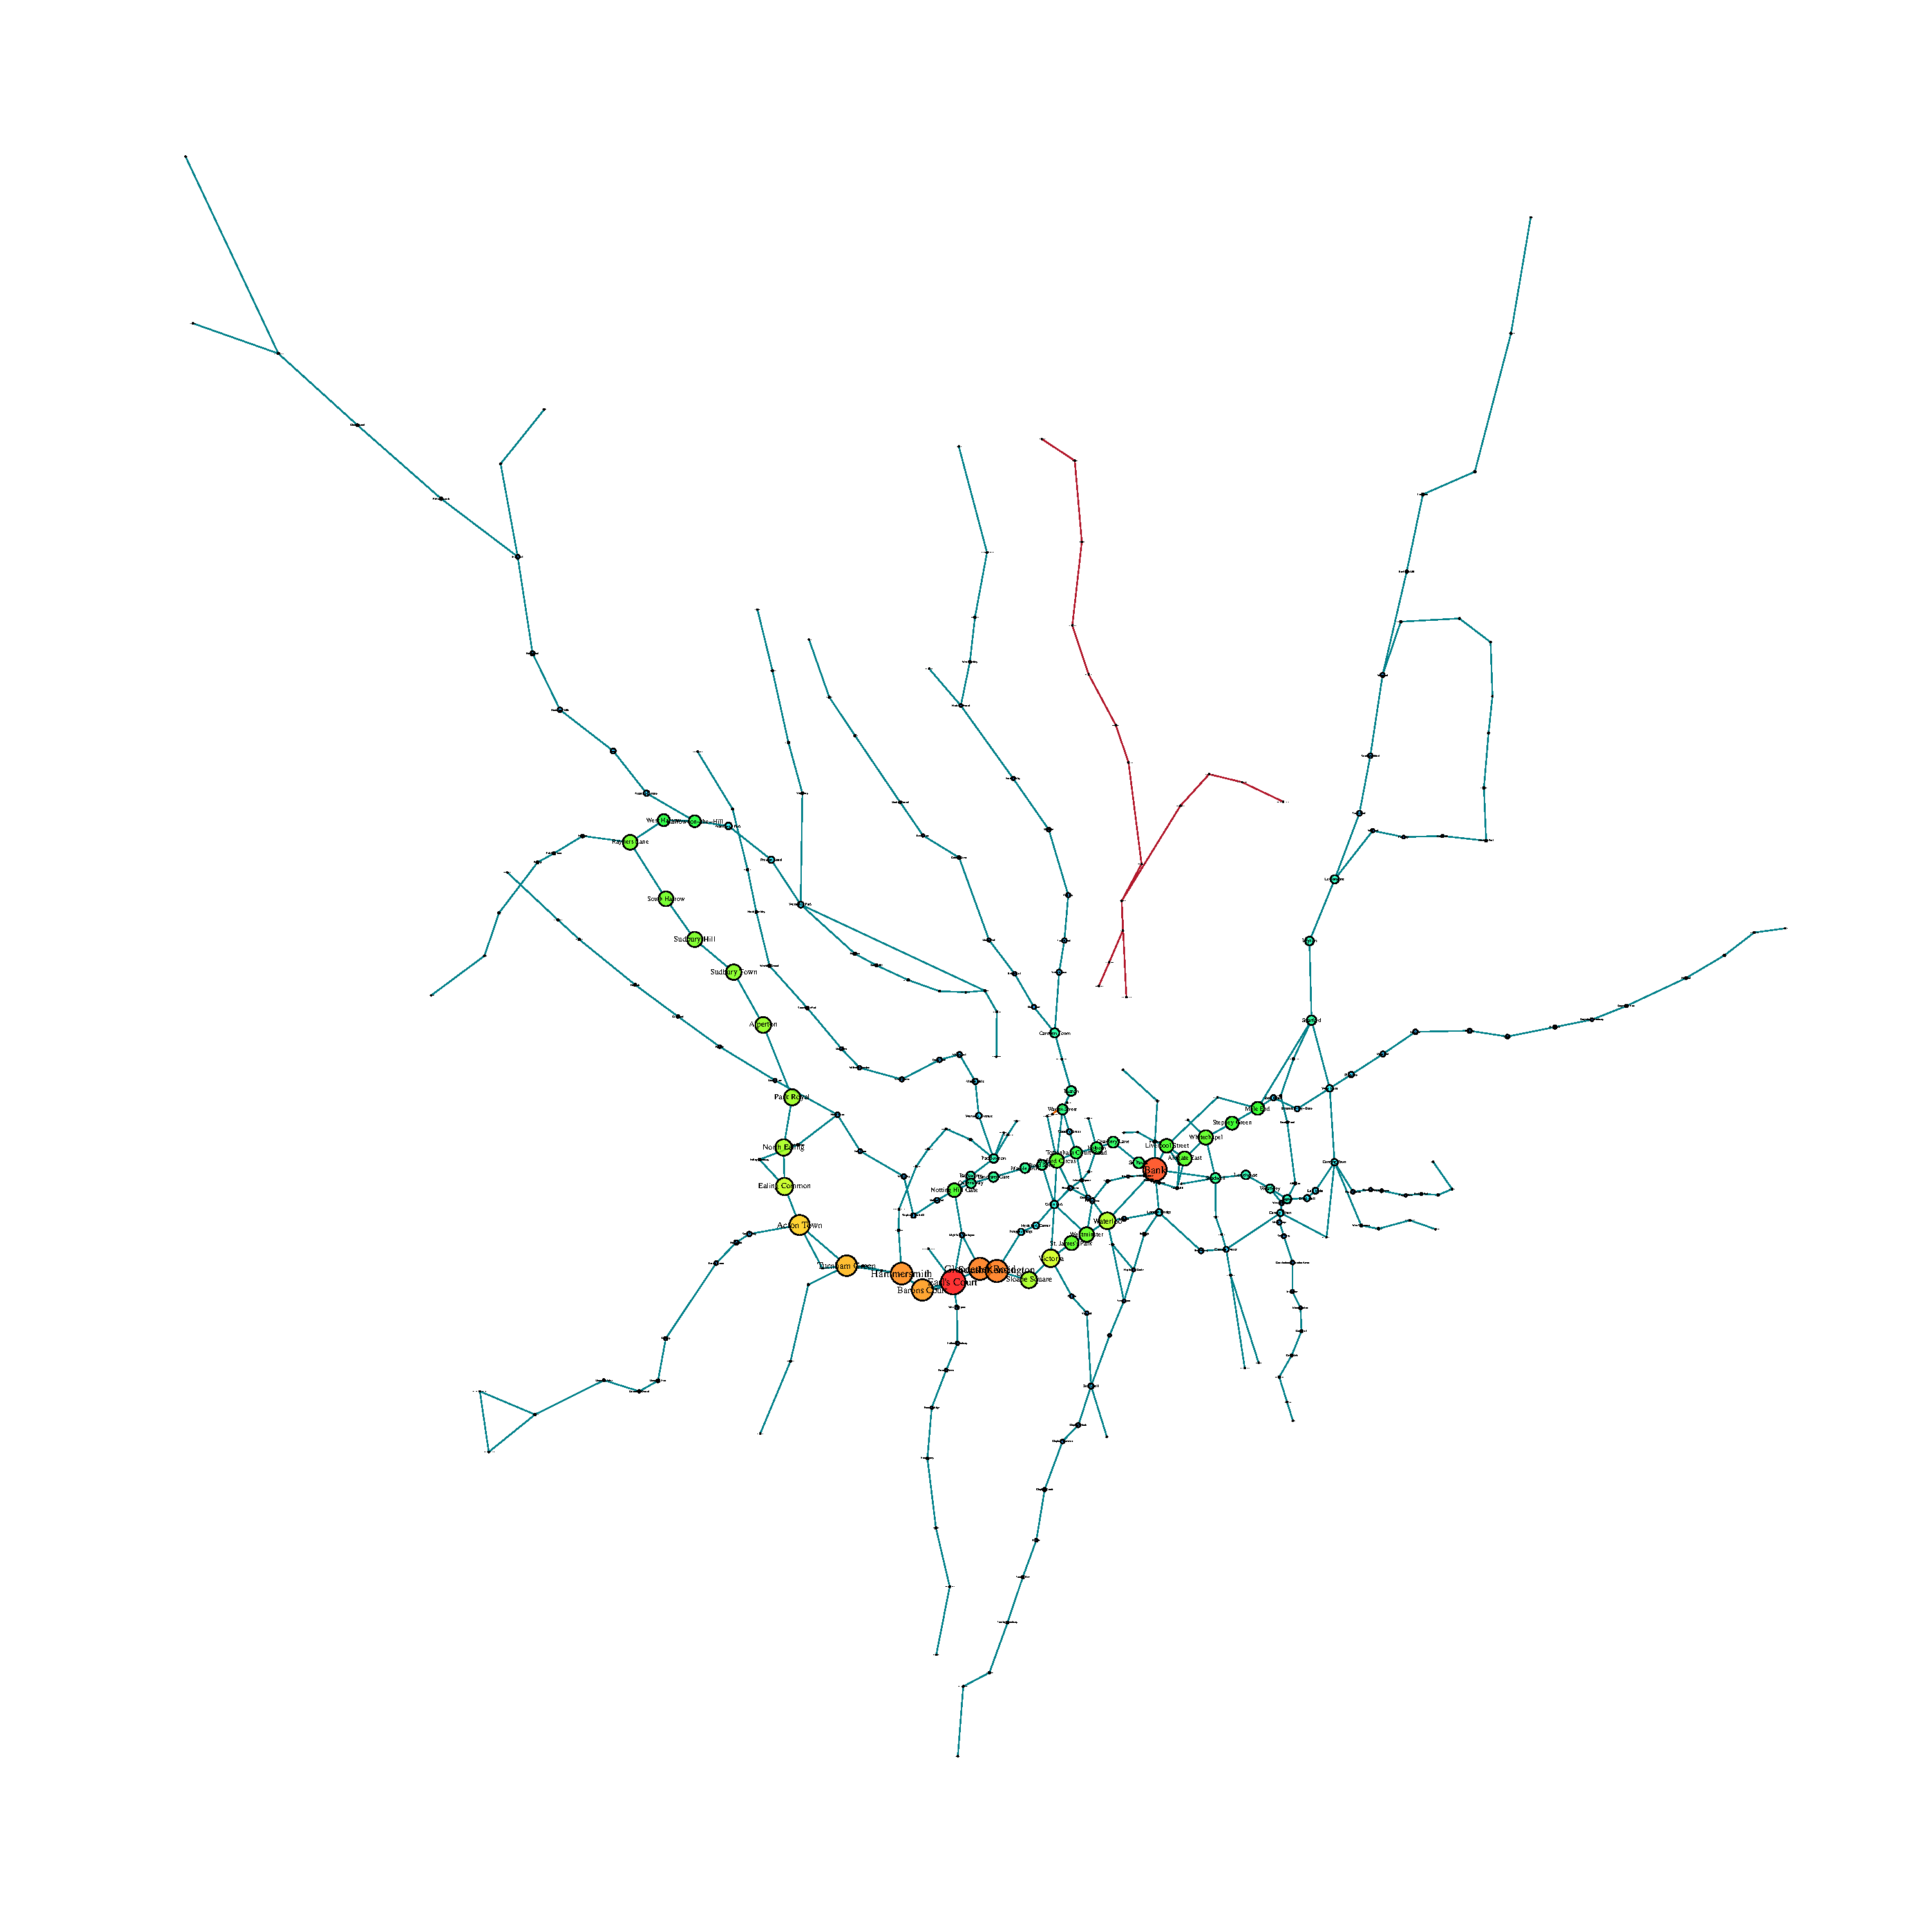
\includegraphics[clip, trim=3cm 3cm 0.25cm 2cm,width=1\textwidth]{images/NW/2_1.pdf}
    \caption{The topographical map of the London underground network after removing King's Cross St. Pancras and Baker Street}\label{fig: 2_1}
\end{minipage}
\begin{minipage}[b]{0.5\textwidth}
\centering
    \captionsetup{width=.9\linewidth}
    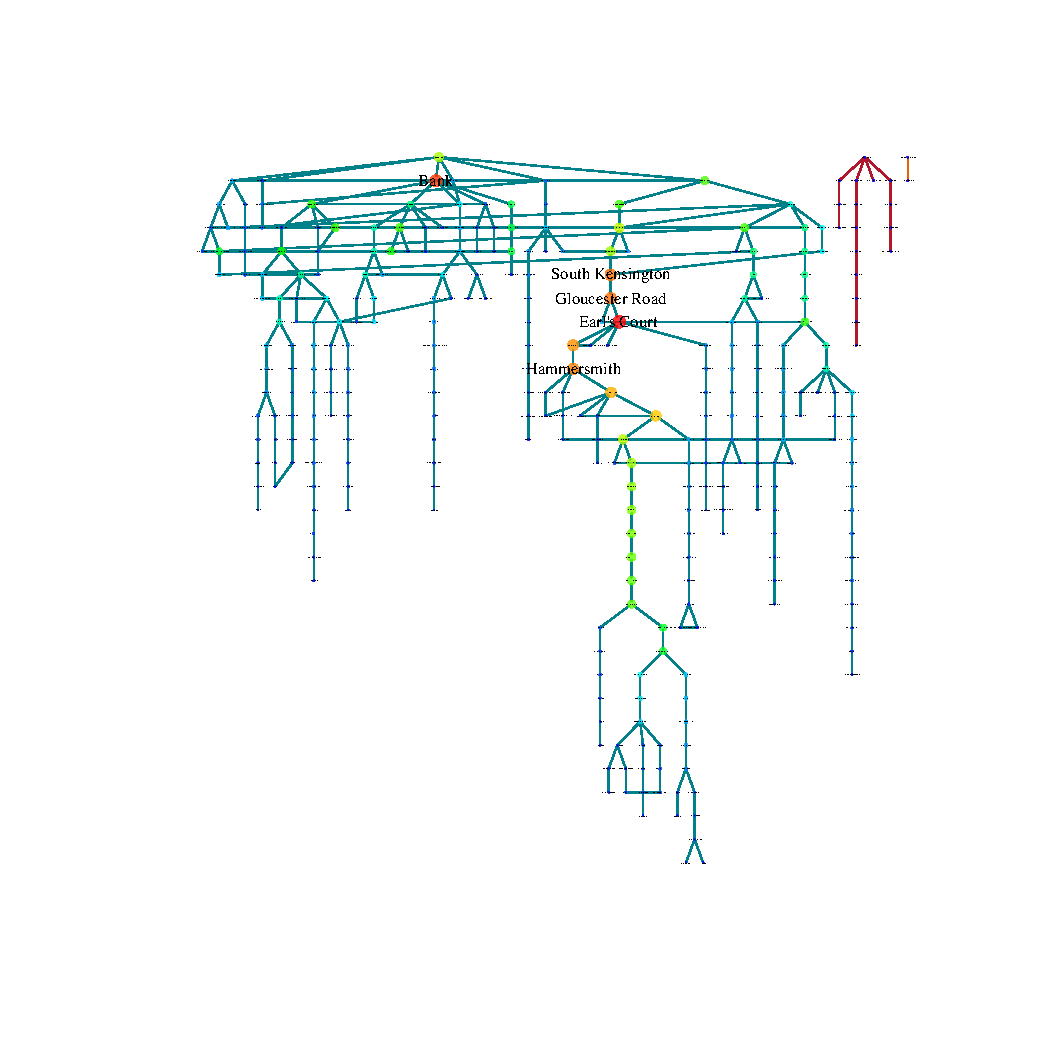
\includegraphics[clip, trim=3cm 3cm 0.25cm 2cm,width=1\textwidth]{images/NW/2_2.pdf}
    \caption{The tree topology of the London underground network after removing King's Cross St. Pancras and Baker Street}\label{fig: 2_2}
\end{minipage}
\end{figure}  

\subsubsection{Blocking the Most Pathways}
If terrorists' aim is to disrupt stations that allows the most shortest paths to go through, then Baker Street would be the No.1 target. If two stations are chosen, how to choose the combination is difficult. The first option is the top 2 stations on the list: Baker Street and Bank. However, if they choose to disrupt sequentially, the station that has the highest betweeenness centrality would change to Earl's Court after destroying Baker Street. 
\\A major change of the network the removal of Baker Street causes is the move of high betweenness area from center London to the southern part. The combination of two top ranked stations (see figure \ref{fig: 3_1} and \ref{fig: 3_2}) turns out adding very weak influences compared to just removing one station. The choose of removing two stations sequentially gets better results by creating an addition components (See figure \ref{fig: 5_1} and \ref{fig: 5_2}).
\begin{figure}[H]
\centering
\begin{minipage}[b]{0.49\textwidth}
\centering
    \captionsetup{width=.9\linewidth}
    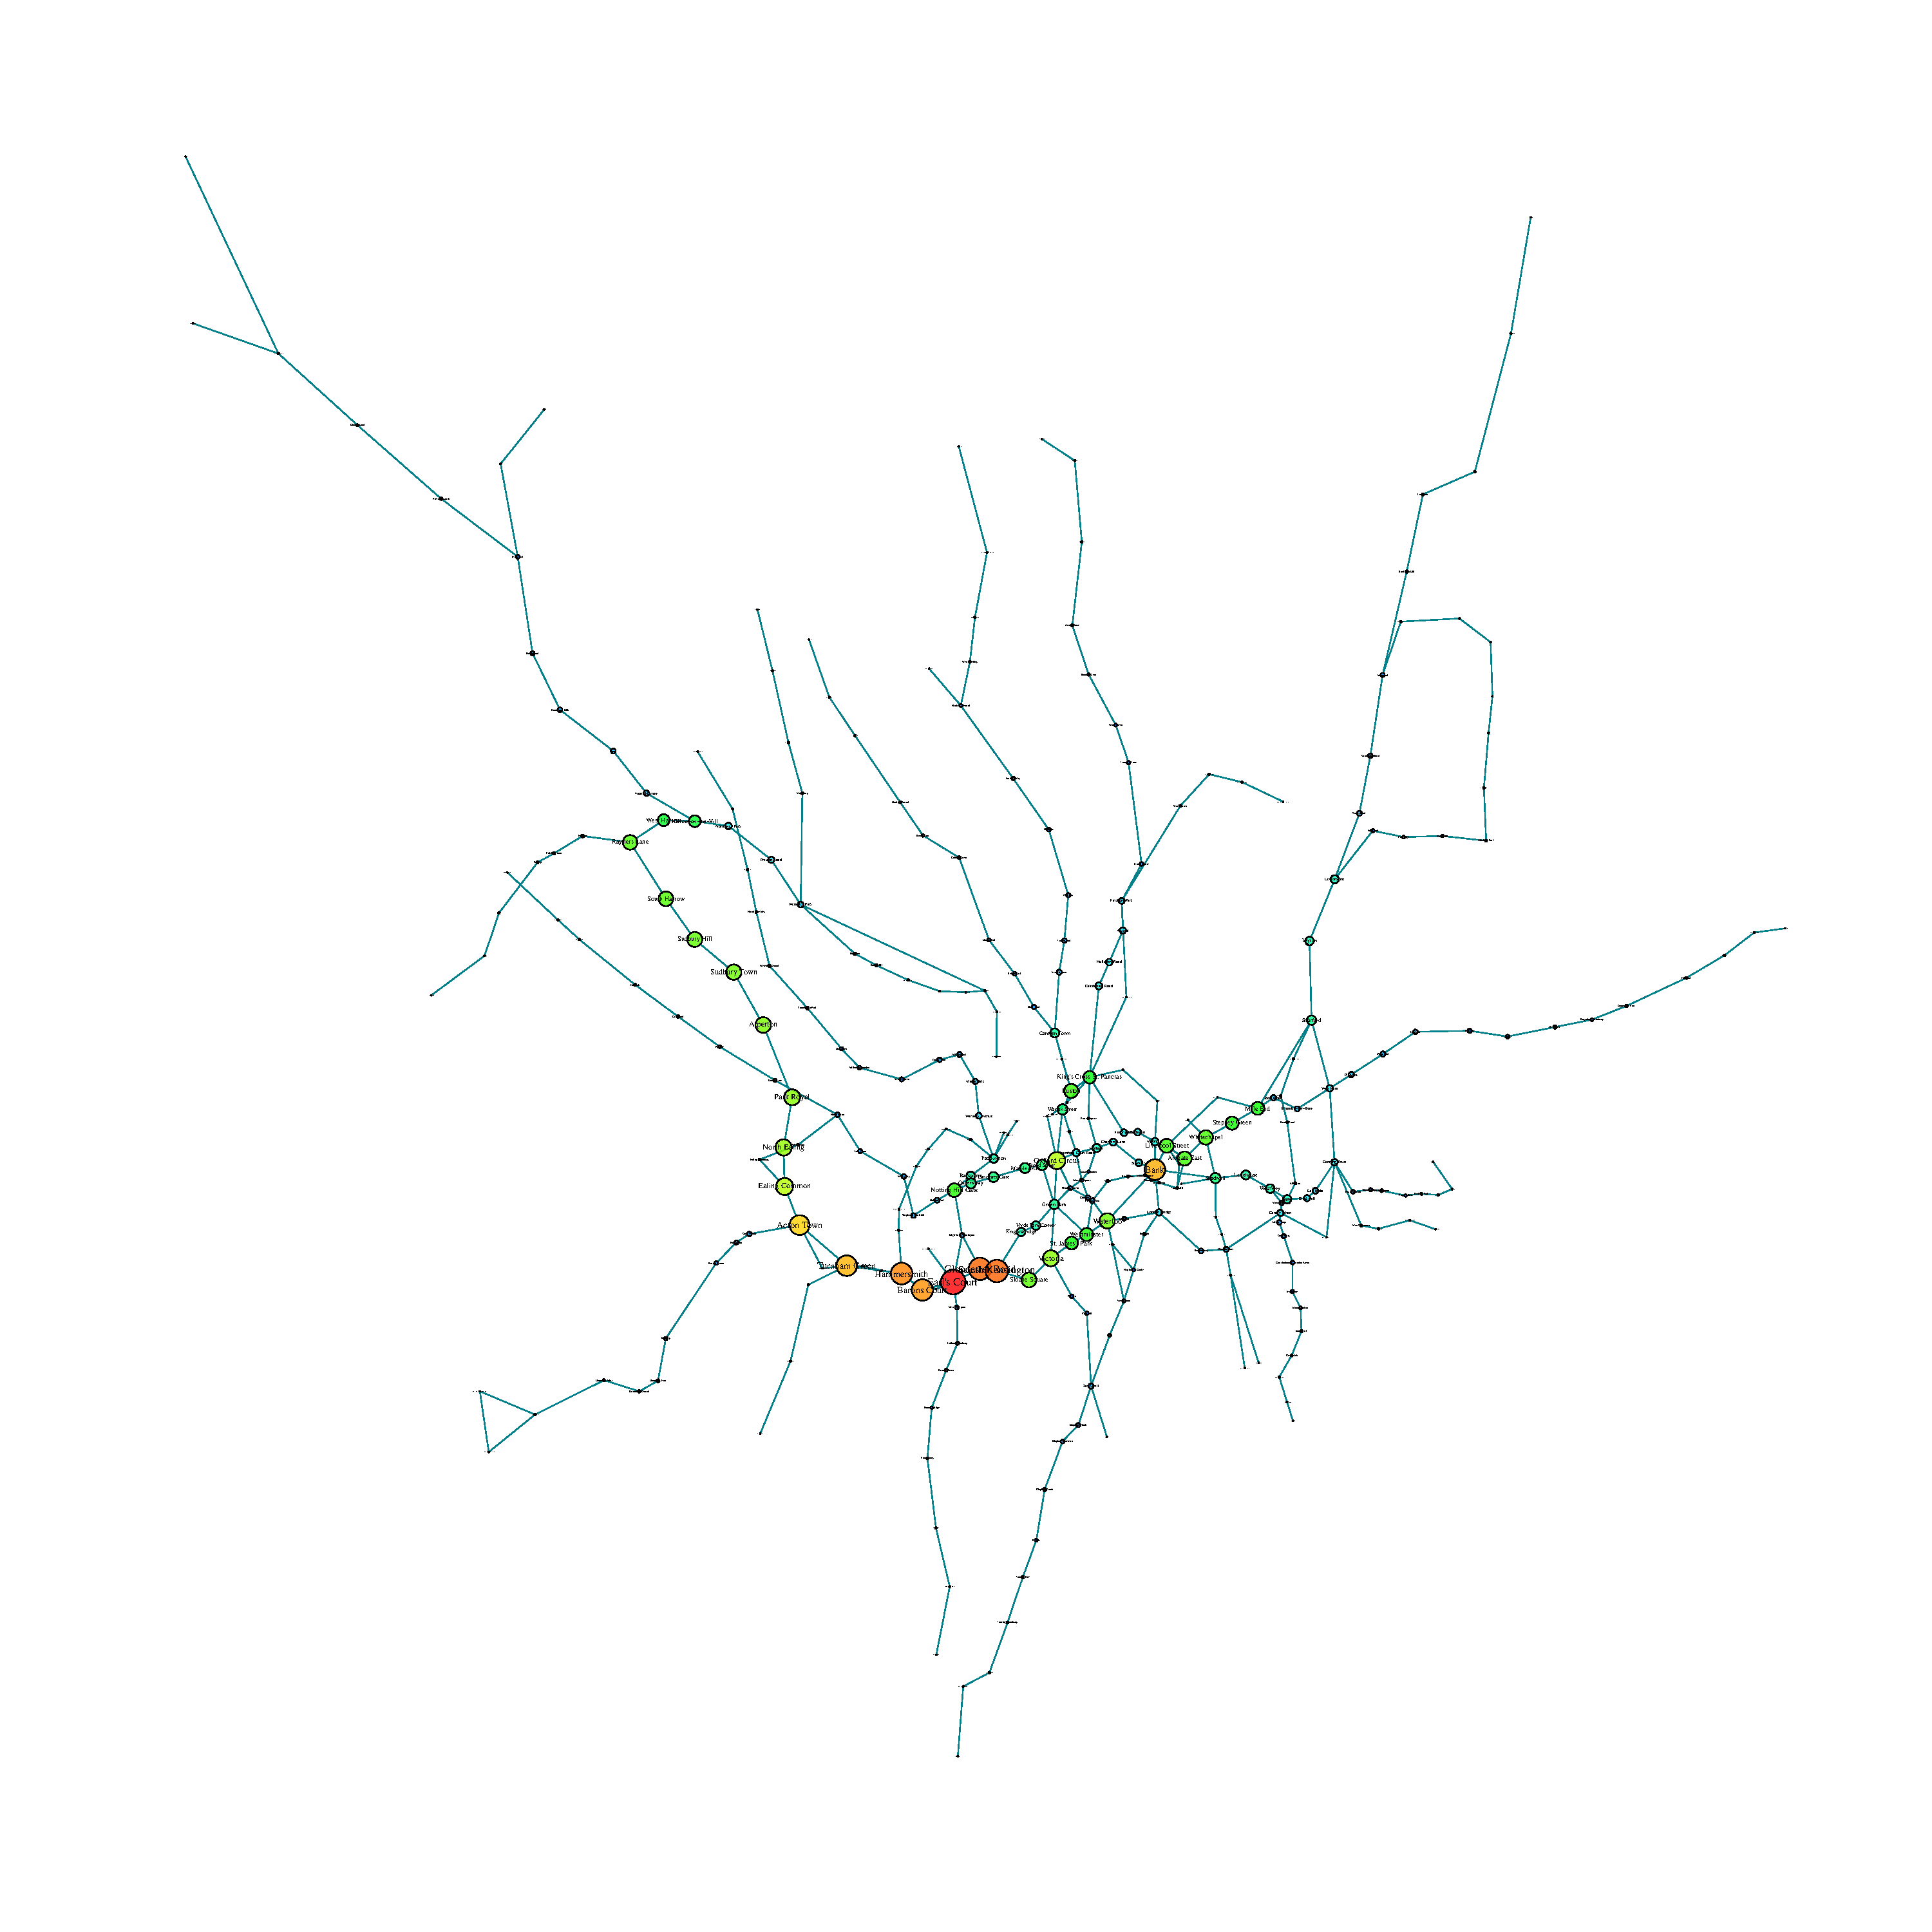
\includegraphics[clip, trim=3cm 3cm 3cm 2cm,width=1\textwidth]{images/NW/3_1.pdf}
    \caption{The topographical map of the London underground network removing Baker Street}\label{fig: 3_1}
\end{minipage}
\begin{minipage}[b]{0.5\textwidth}
\centering
    \captionsetup{width=.9\linewidth}
    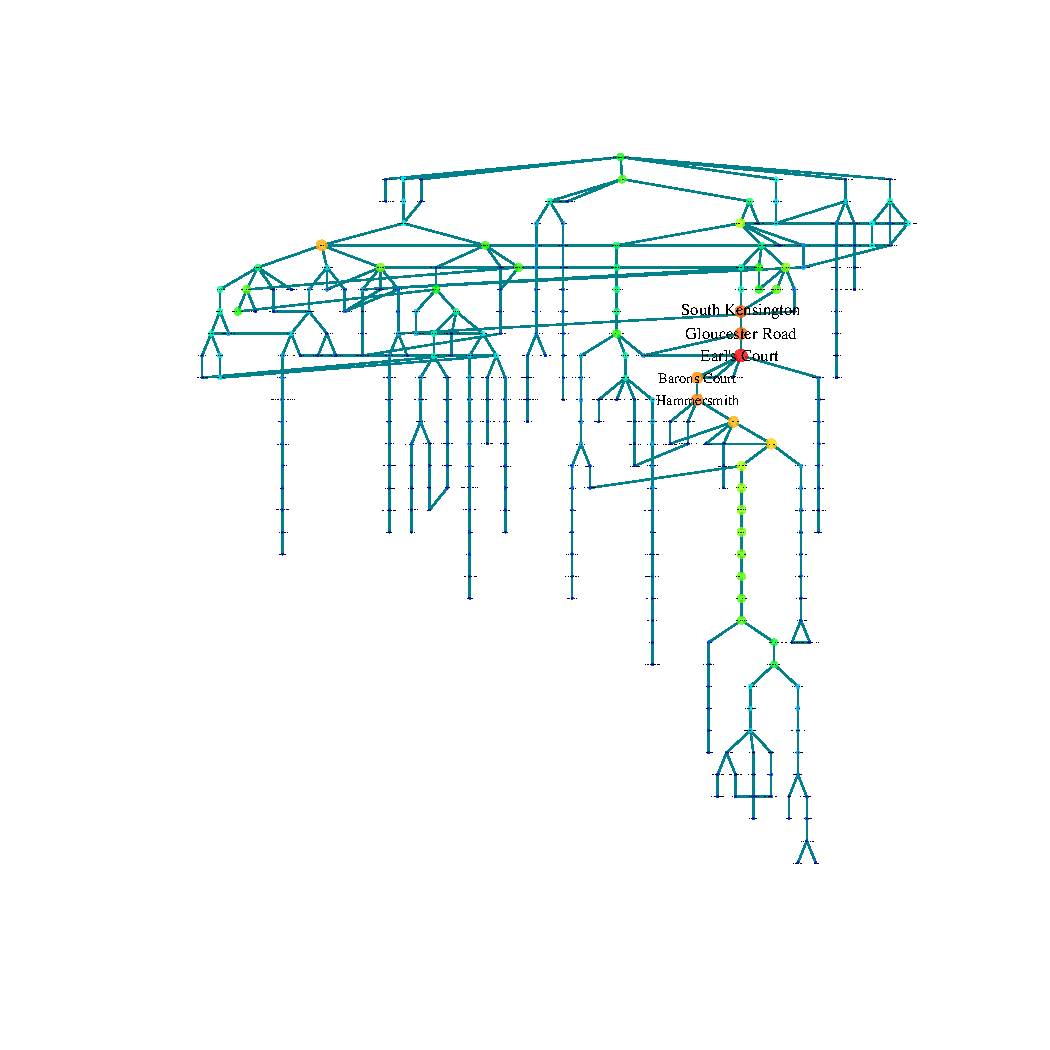
\includegraphics[clip, trim=3cm 3cm 3cm 2cm,width=1\textwidth]{images/NW/3_2.pdf}
    \caption{The tree topology of the London underground network after removing Baker Street}\label{fig: 3_2}
\end{minipage}
\end{figure} 
\begin{figure}[H]
\centering
\begin{minipage}[b]{0.49\textwidth}
\centering
    \captionsetup{width=.9\linewidth}
    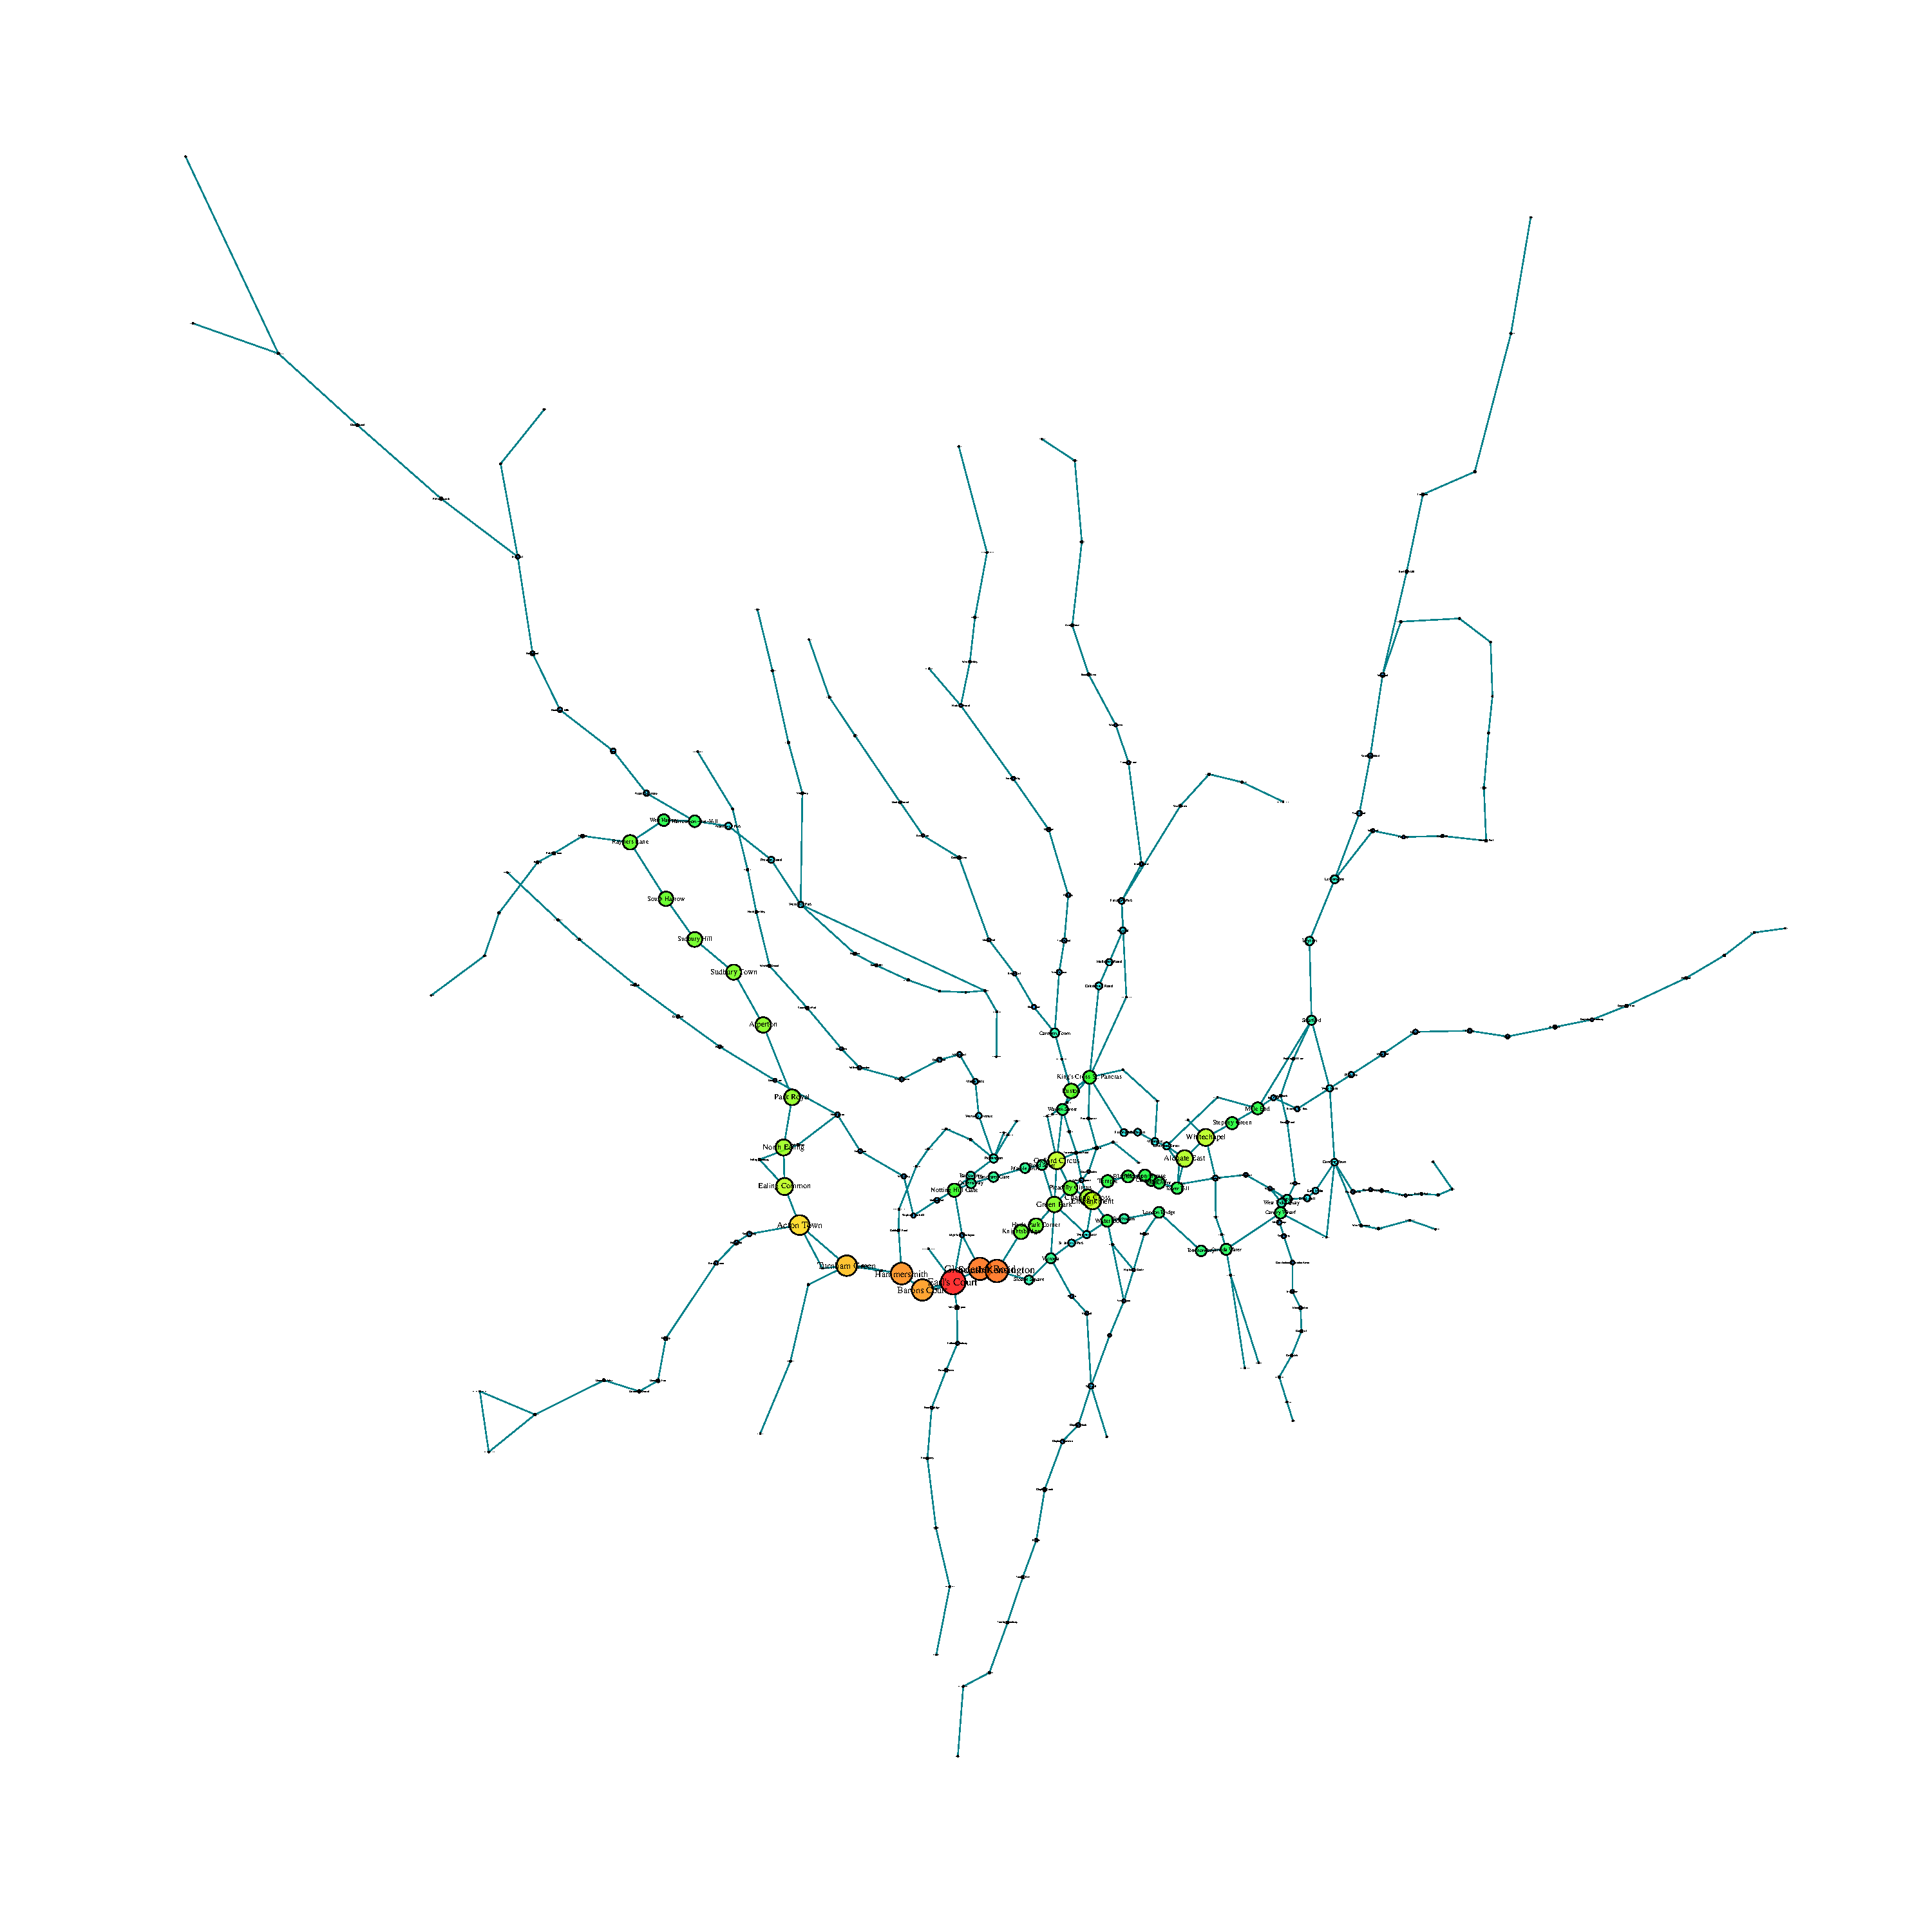
\includegraphics[clip, trim=3cm 3cm 3cm 2cm,width=1\textwidth]{images/NW/4_1.pdf}
    \caption{The topographical map of the London underground network removing Baker Street and Bank}\label{fig: 4_1}
\end{minipage}
\begin{minipage}[b]{0.5\textwidth}
\centering
    \captionsetup{width=.9\linewidth}
    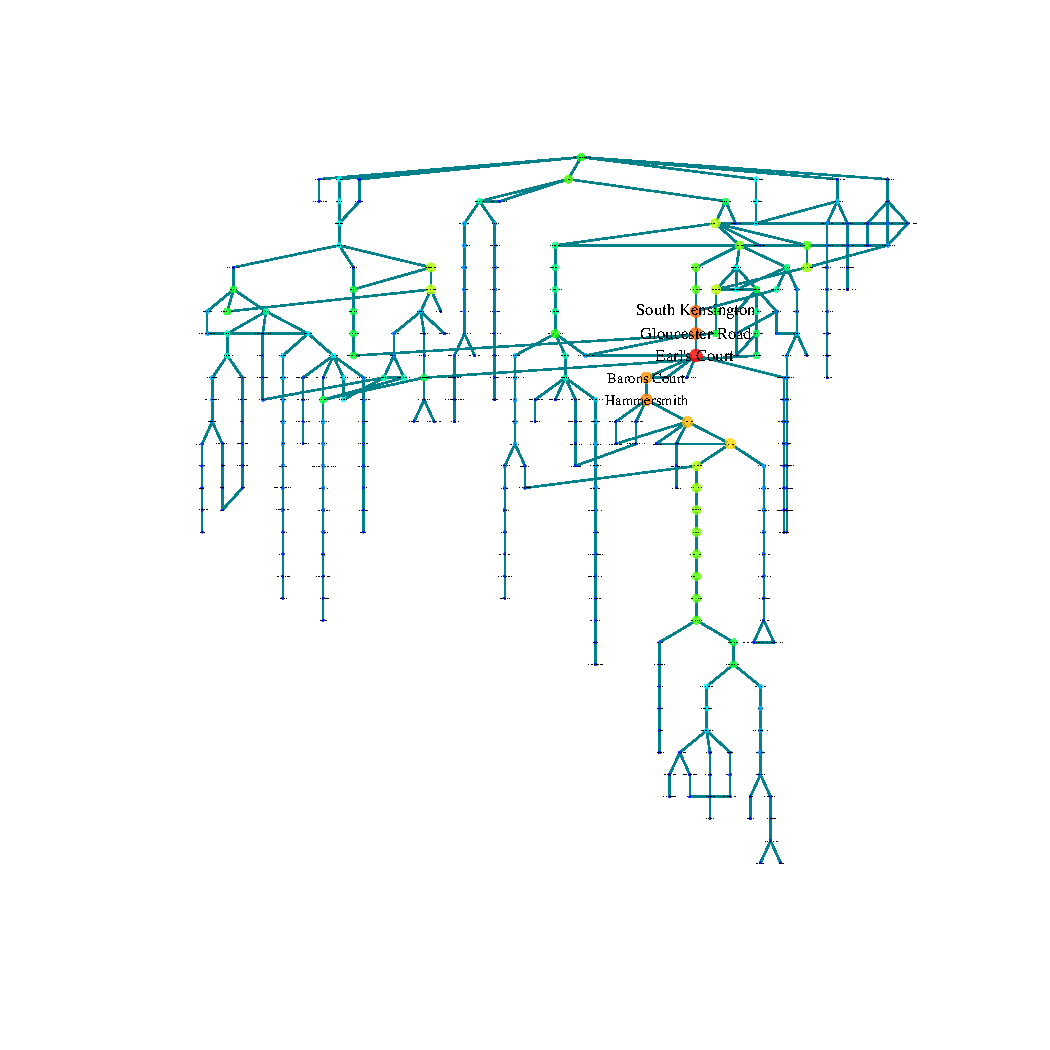
\includegraphics[clip, trim=3cm 3cm 2cm 2cm,width=1\textwidth]{images/NW/4_2.pdf}
    \caption{The tree topology of the London underground network after removing Baker Street and Bank}\label{fig: 4_2}
\end{minipage}
\end{figure} 
\begin{figure}[H]
\centering
\begin{minipage}[b]{0.49\textwidth}
\centering
    \captionsetup{width=.9\linewidth}
    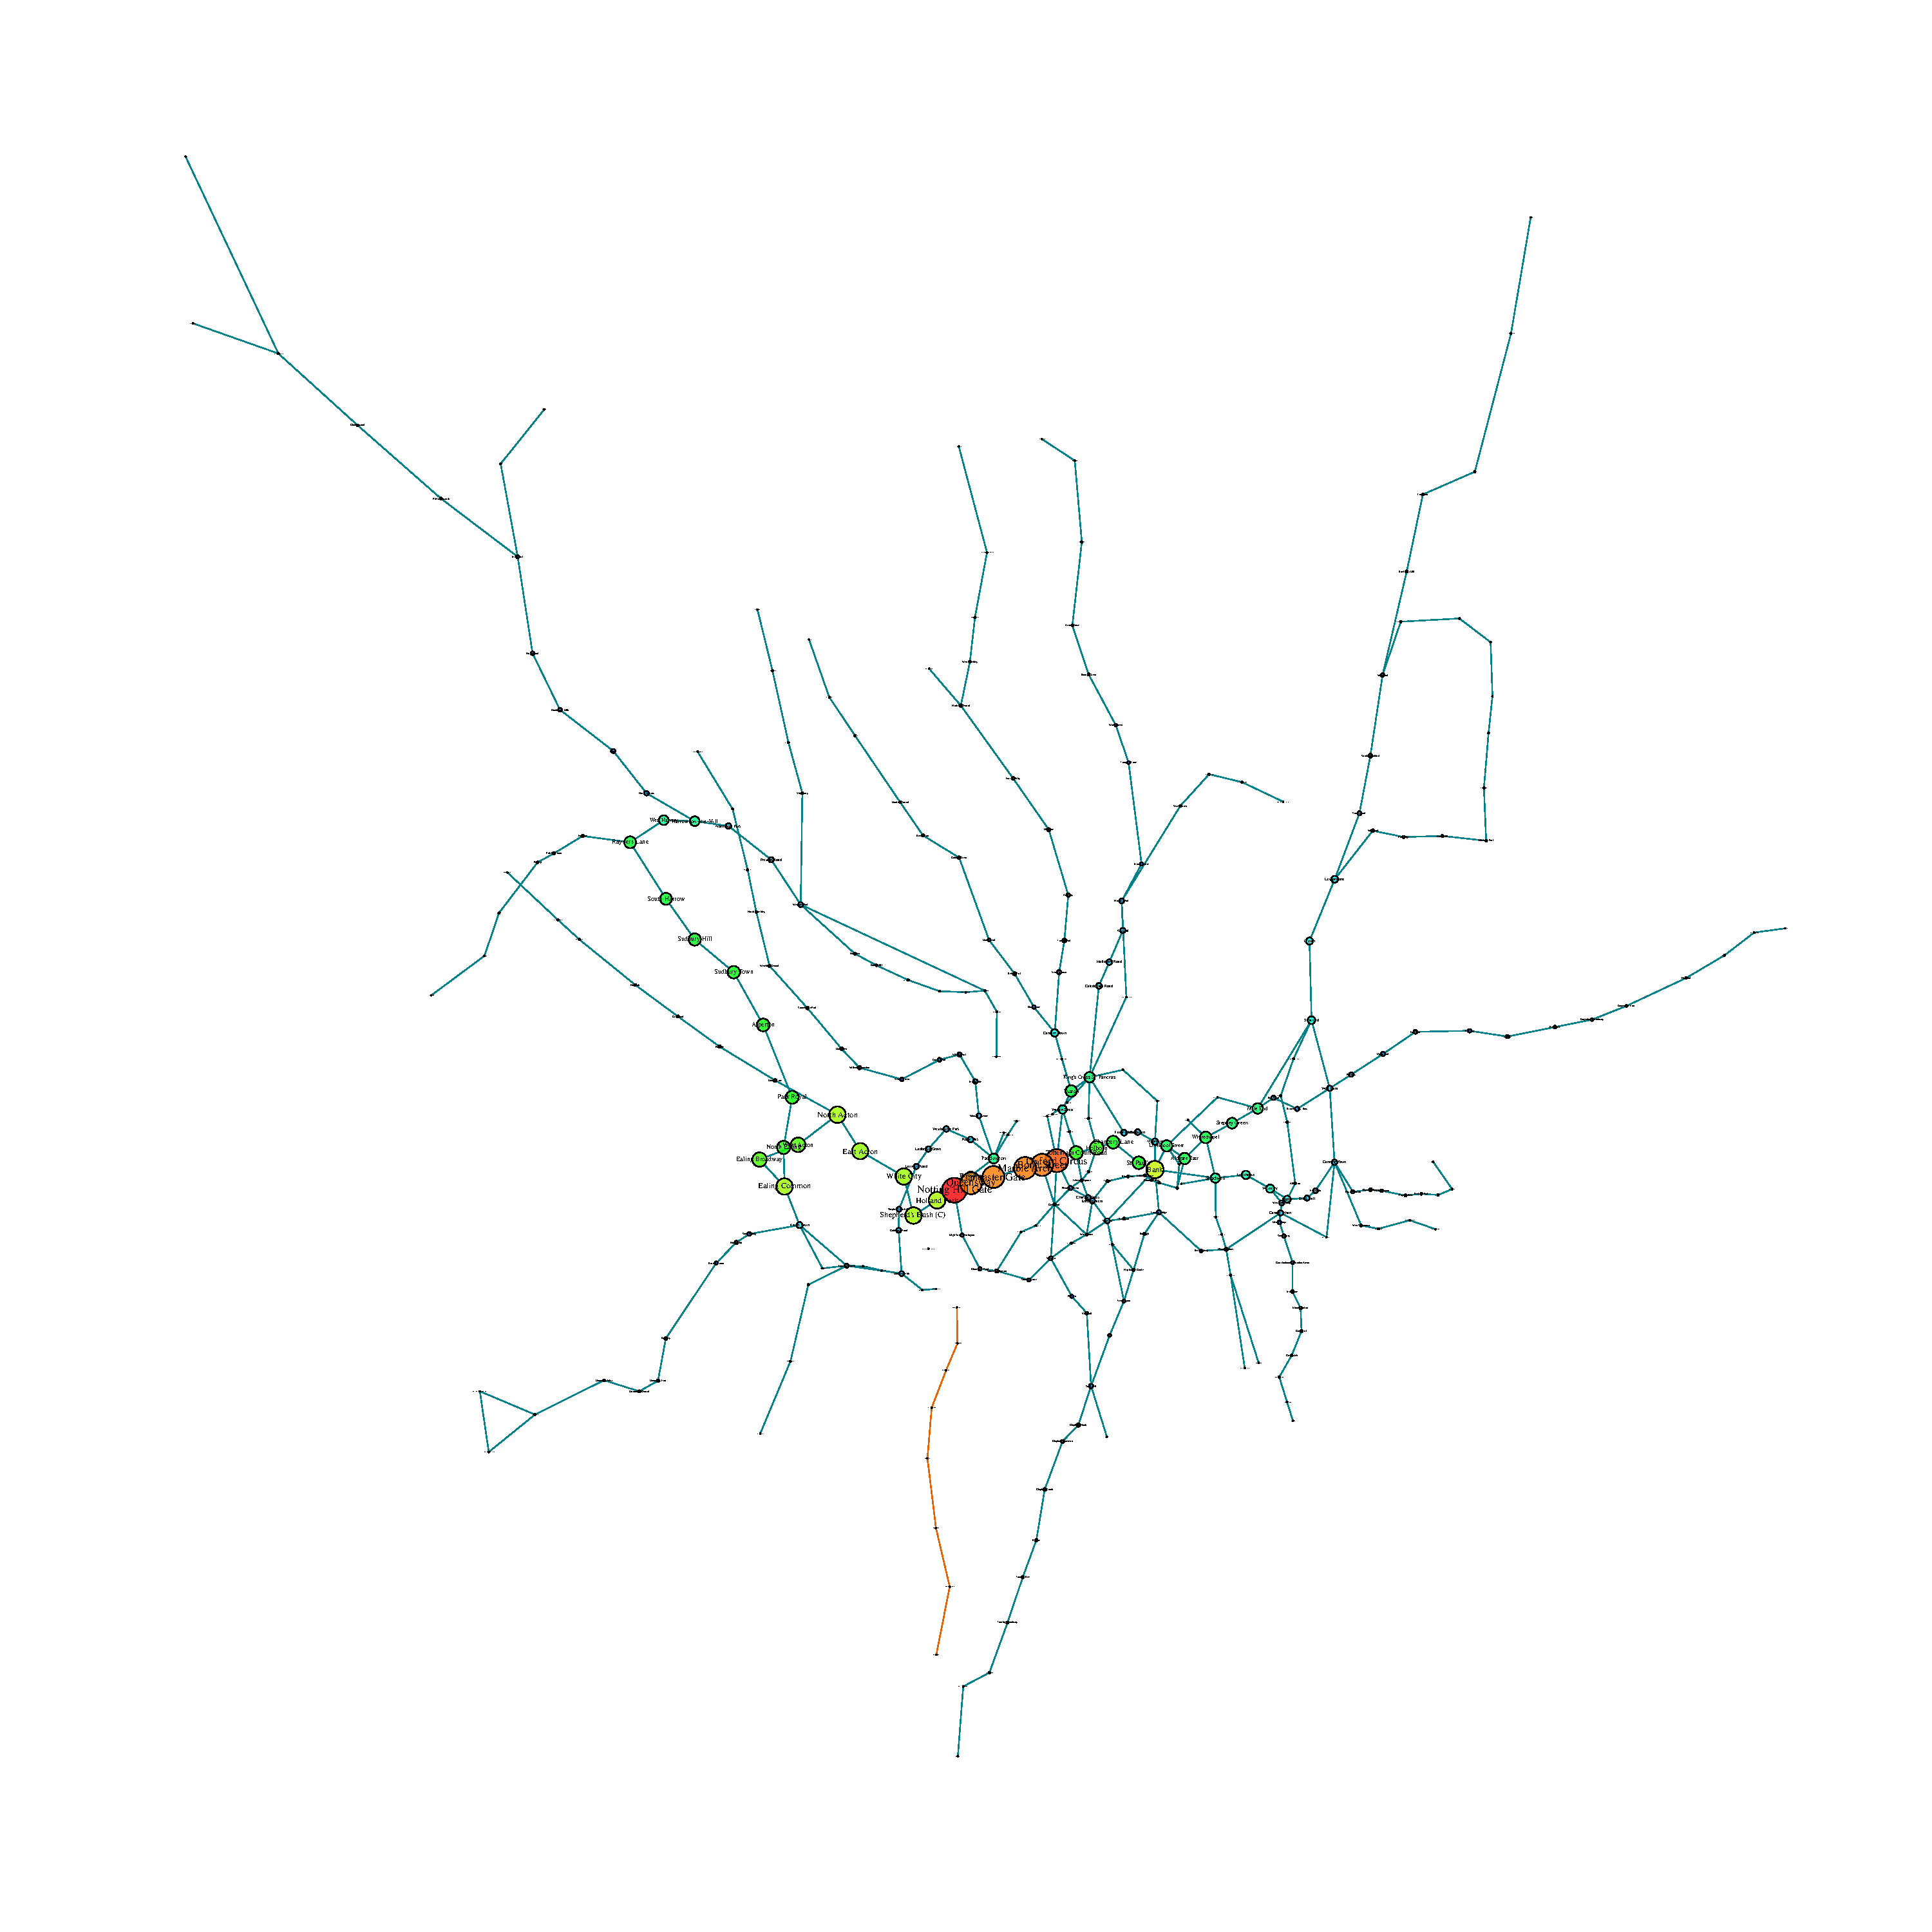
\includegraphics[clip, trim=3cm 3cm 3cm 2cm,width=1\textwidth]{images/NW/5_1.pdf}
    \caption{The topographical map of the London underground network after removing Baker Street and Earl's Court}\label{fig: 5_1}
\end{minipage}
\begin{minipage}[b]{0.5\textwidth}
\centering
    \captionsetup{width=.9\linewidth}
    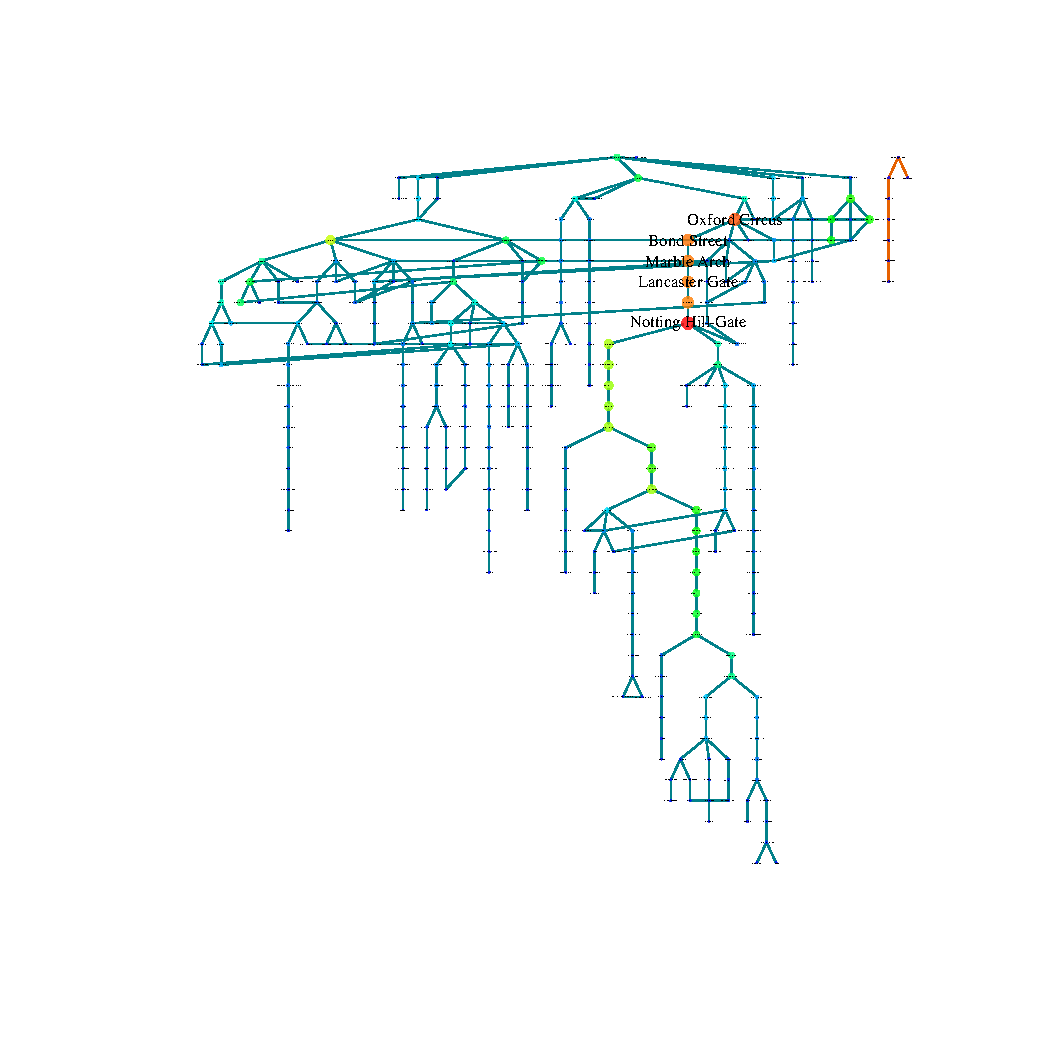
\includegraphics[clip, trim=3cm 3cm 2cm 2cm,width=1\textwidth]{images/NW/5_2.pdf}
    \caption{The tree topology of the London underground network after removing Baker Street and Earl's Court}\label{fig: 5_2}
\end{minipage}
\end{figure} 

\subsubsection{Fragmenting the Whole Tube Network}
If terrorists plan to fragment the whole tube system as much as possible, several aspects are required to be taken into consideration. First criteria is the ability of node to divided the network into parts. Second, it is better to disconnect the network into two rough equal size; Third, the internal structure of each components is also important. The more discrete it is, the better. Therefore, here fragement centrality is introduced as the measure by calculating the sum of reciprocals of distances (see table \ref{tab:keystation2}).
\\The first choice is Baker Street which has already been analysed above. When it comes to two targets, there are 46665 options to pick up two different nodes from all the 306 nodes. Kpset method is applied by using keyplayer package in R. It turns out that the combination of Baker Street and  Ealing Common is the optimal one. 
\\If three stations are chosen, the former two stations together with King's Cross St. Pancras is the best result that fragments the whole underground network most severely.
From figure \ref{fig: 6_1} and \ref{fig: 6_2}, it can be seen that one critical change compared to the previous two-station selection cases is the size of the smaller components gets bigger, thus making the network more discrete. 
\\The last model removes three stations dividing the network into four sub-networks, the structure of which is the most discrete (see figure \ref{fig: 7_1} and \ref{fig: 7_2}).
\begin{figure}[H]
\centering
\begin{minipage}[b]{0.49\textwidth}
\centering
    \captionsetup{width=.9\linewidth}
    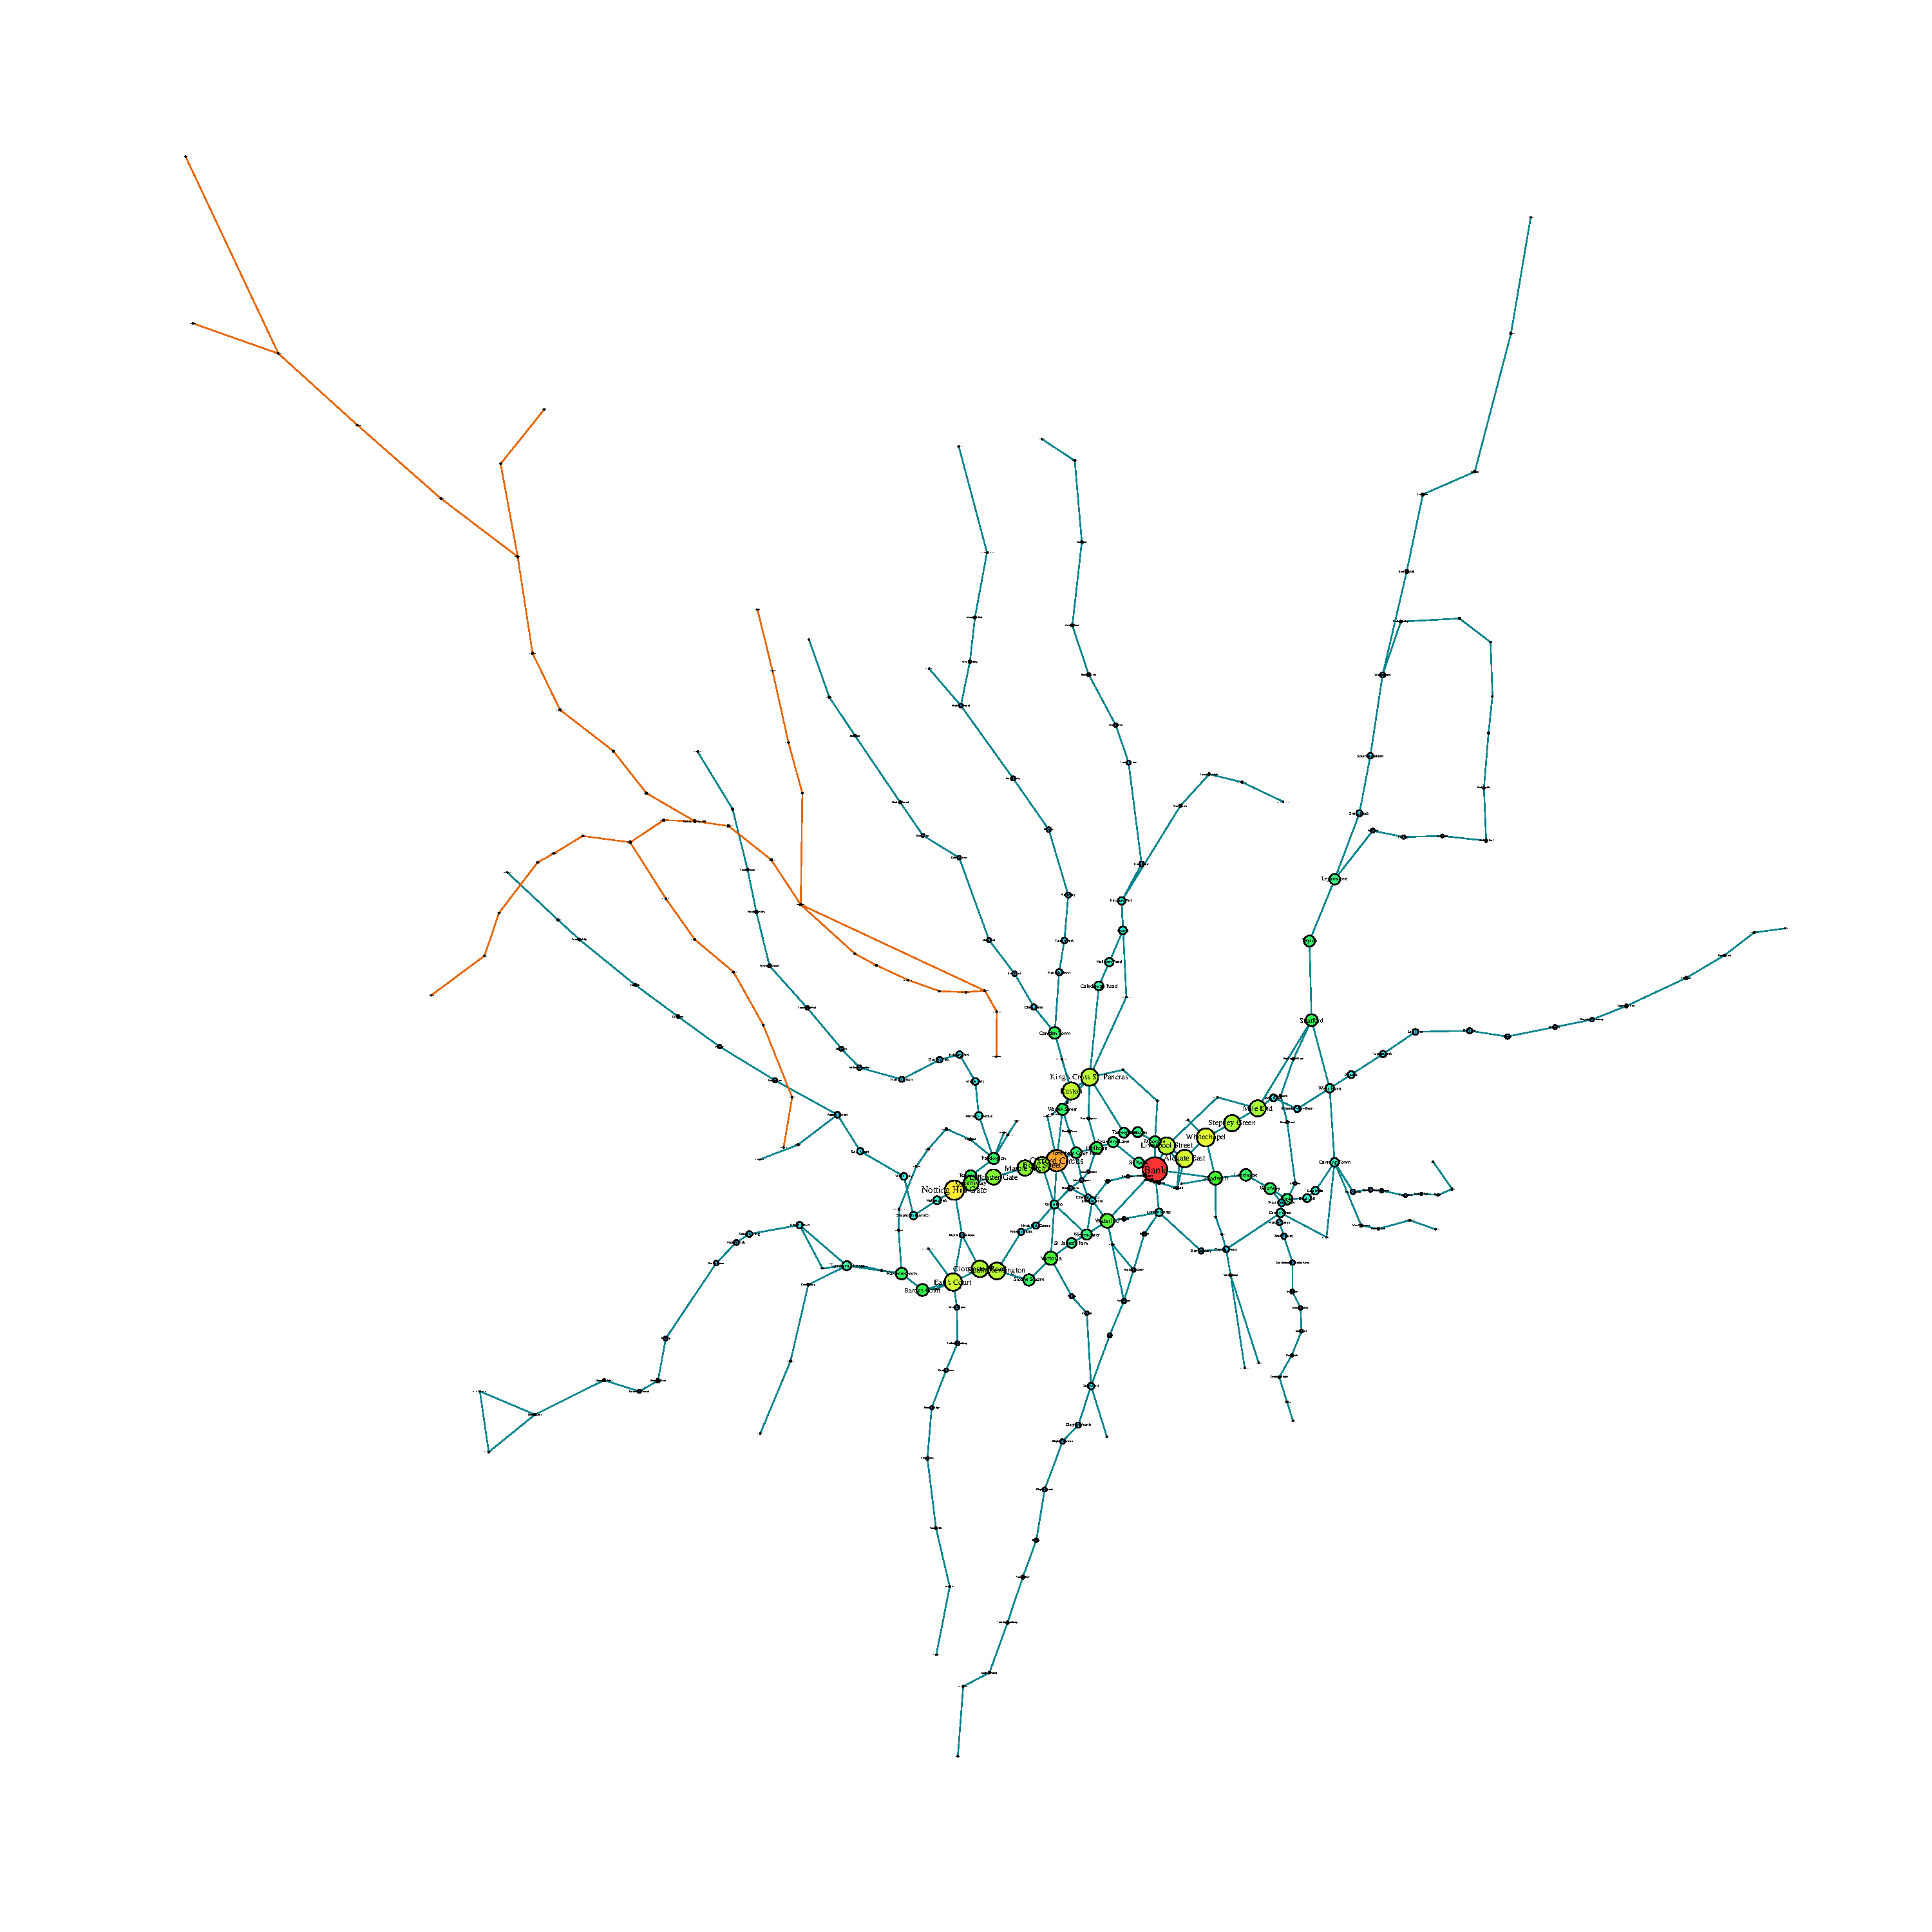
\includegraphics[clip, trim=3cm 3cm 3cm 2cm,width=1\textwidth]{images/NW/6_1.pdf}
    \caption{The topographical map of the London underground network after removing Baker Street and Ealing Common}\label{fig: 6_1}
\end{minipage}
\begin{minipage}[b]{0.5\textwidth}
\centering
    \captionsetup{width=.9\linewidth}
    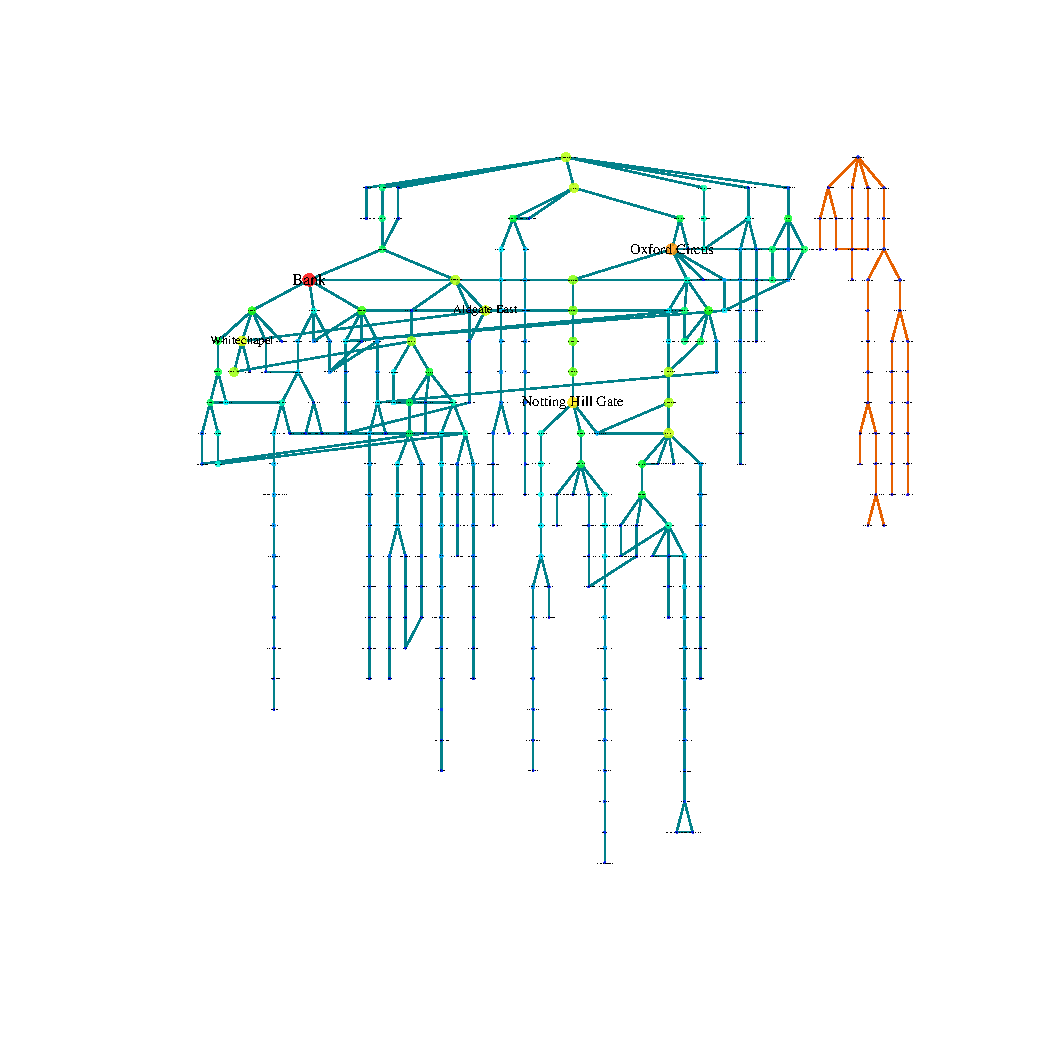
\includegraphics[clip, trim=3cm 3cm 2cm 2cm,width=1\textwidth]{images/NW/6_2.pdf}
    \caption{The tree topology of the London underground network after removing Baker Street and  Ealing Common}\label{fig: 6_2}
\end{minipage}
\end{figure} 
\begin{figure}[H]
\centering
\begin{minipage}[b]{0.49\textwidth}
\centering
    \captionsetup{width=.9\linewidth}
    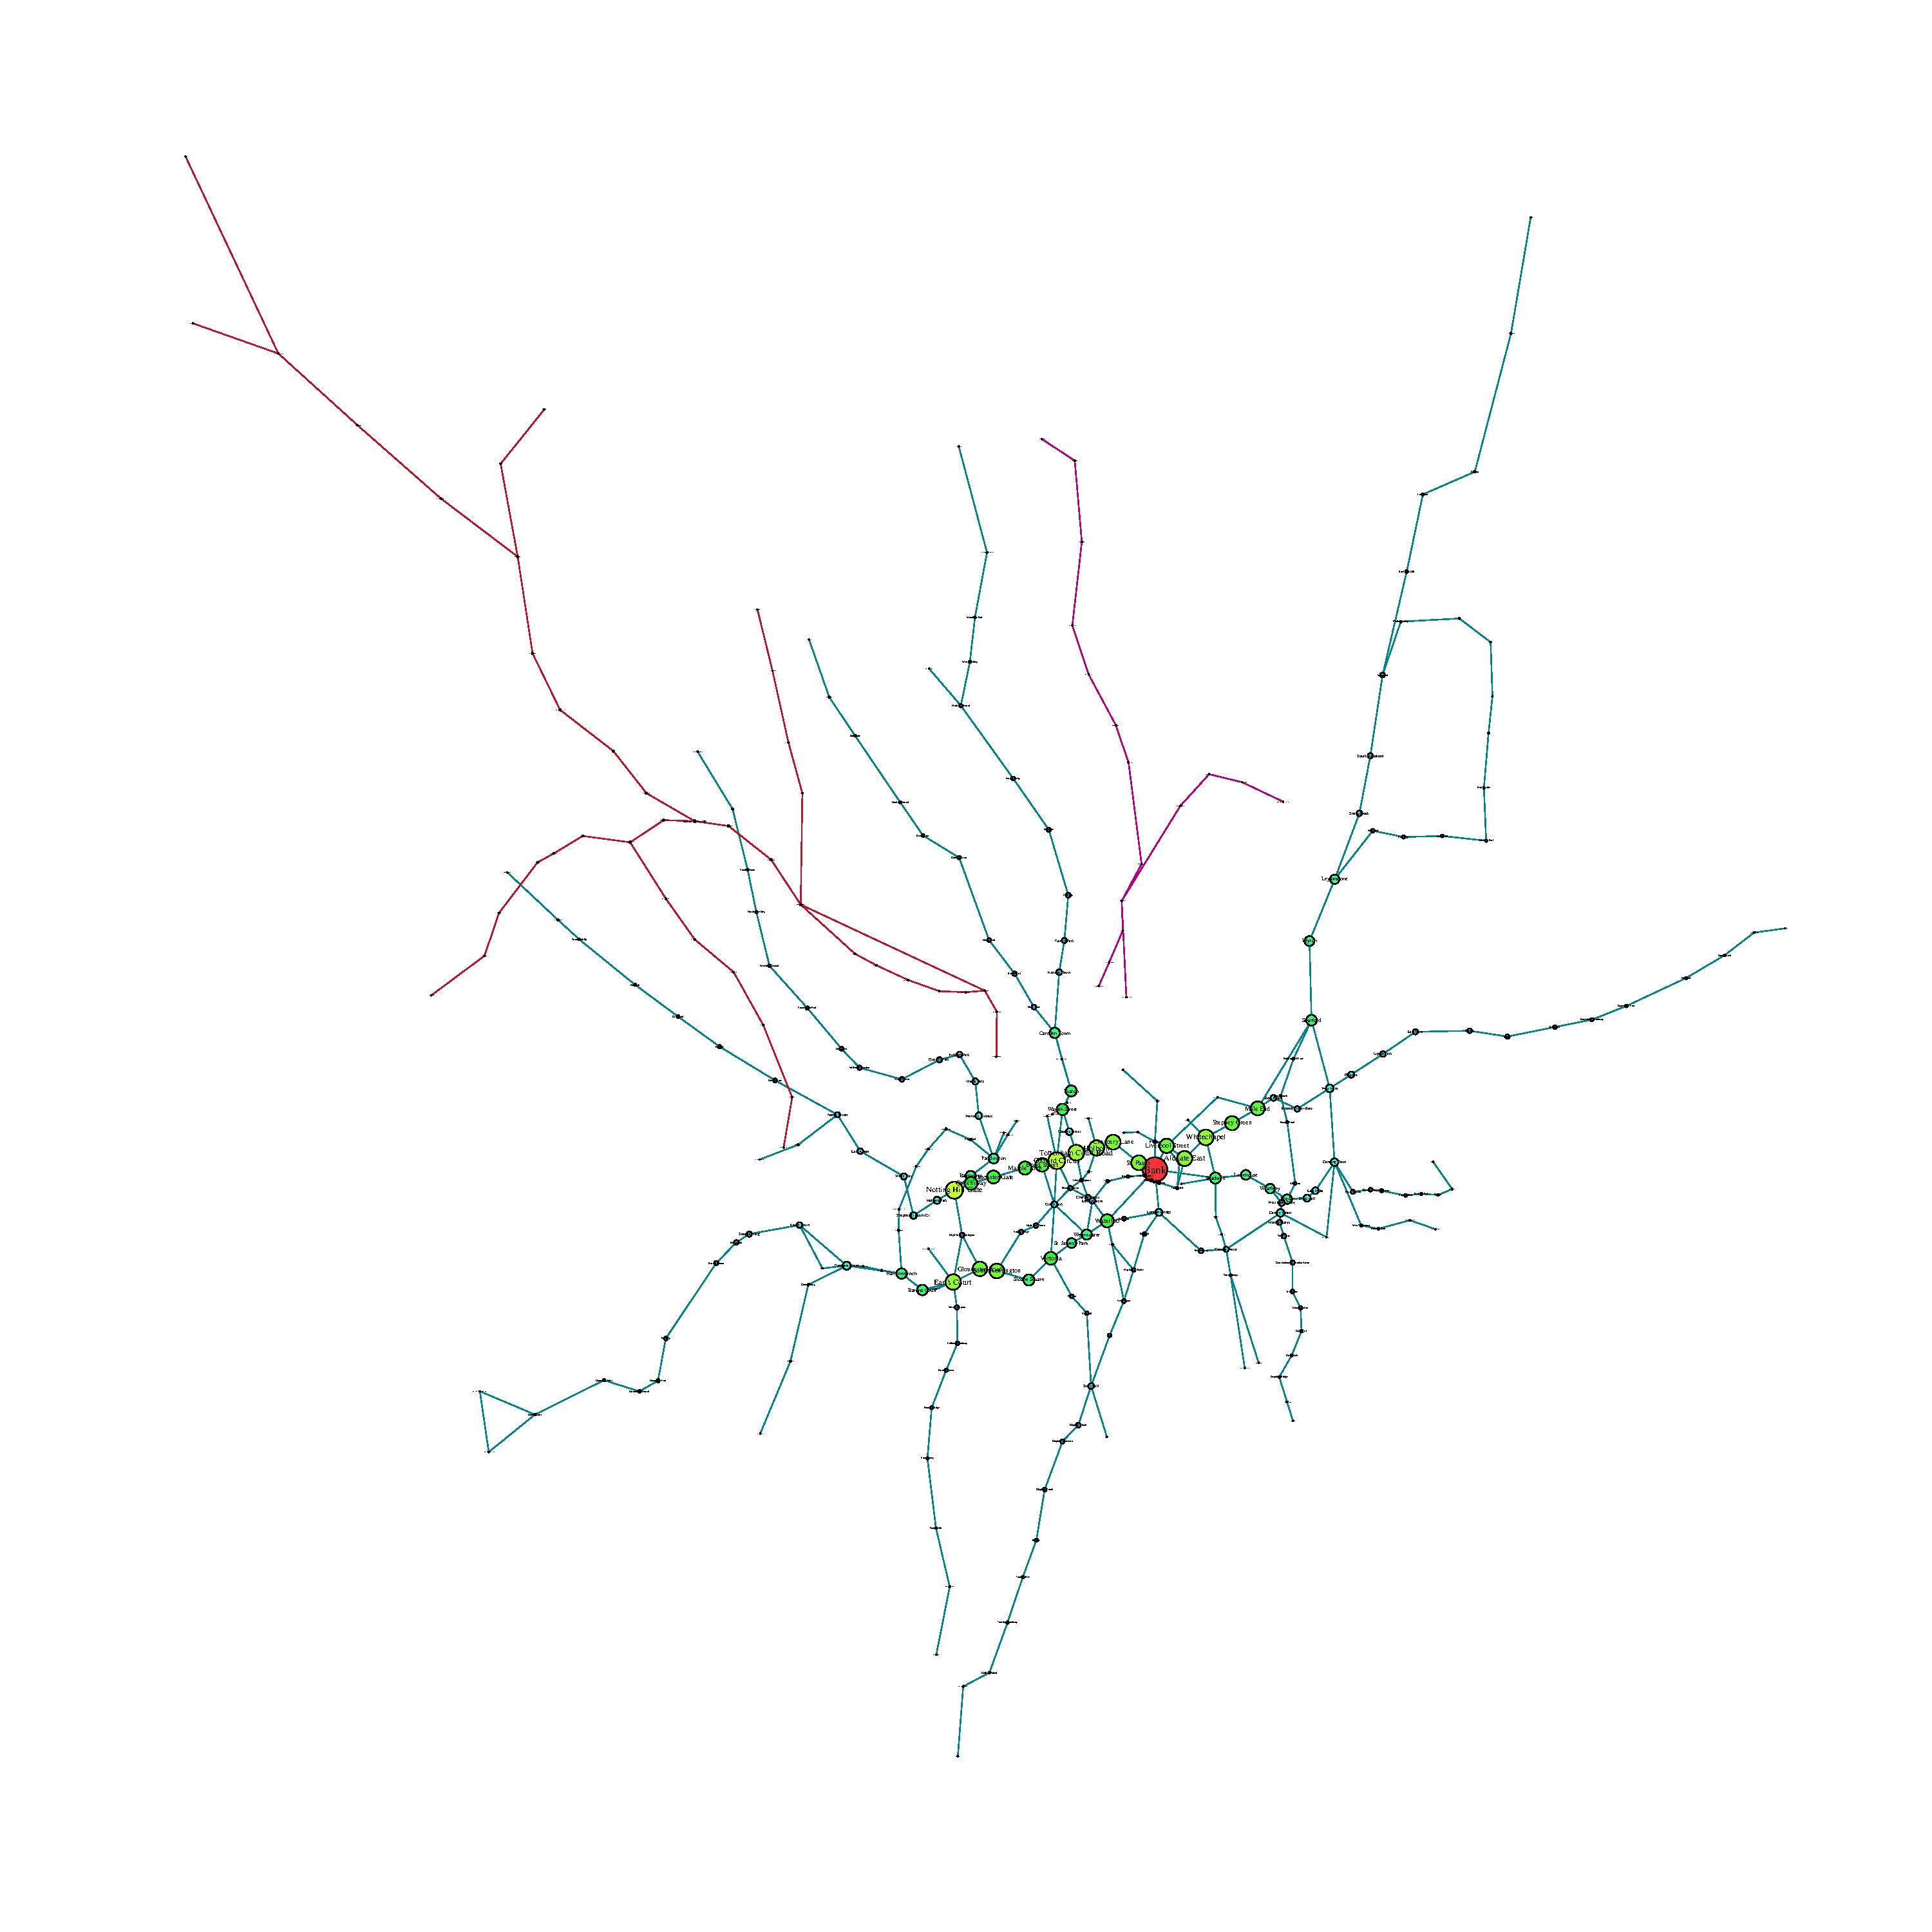
\includegraphics[clip, trim=3cm 3cm 3cm 2cm,width=1\textwidth]{images/NW/7_1.pdf}
    \caption{The topographical map of the London underground network after removing Baker Street, Ealing Common and King's Cross St. Pancras}\label{fig: 7_1}
\end{minipage}
\begin{minipage}[b]{0.5\textwidth}
\centering
    \captionsetup{width=.9\linewidth}
    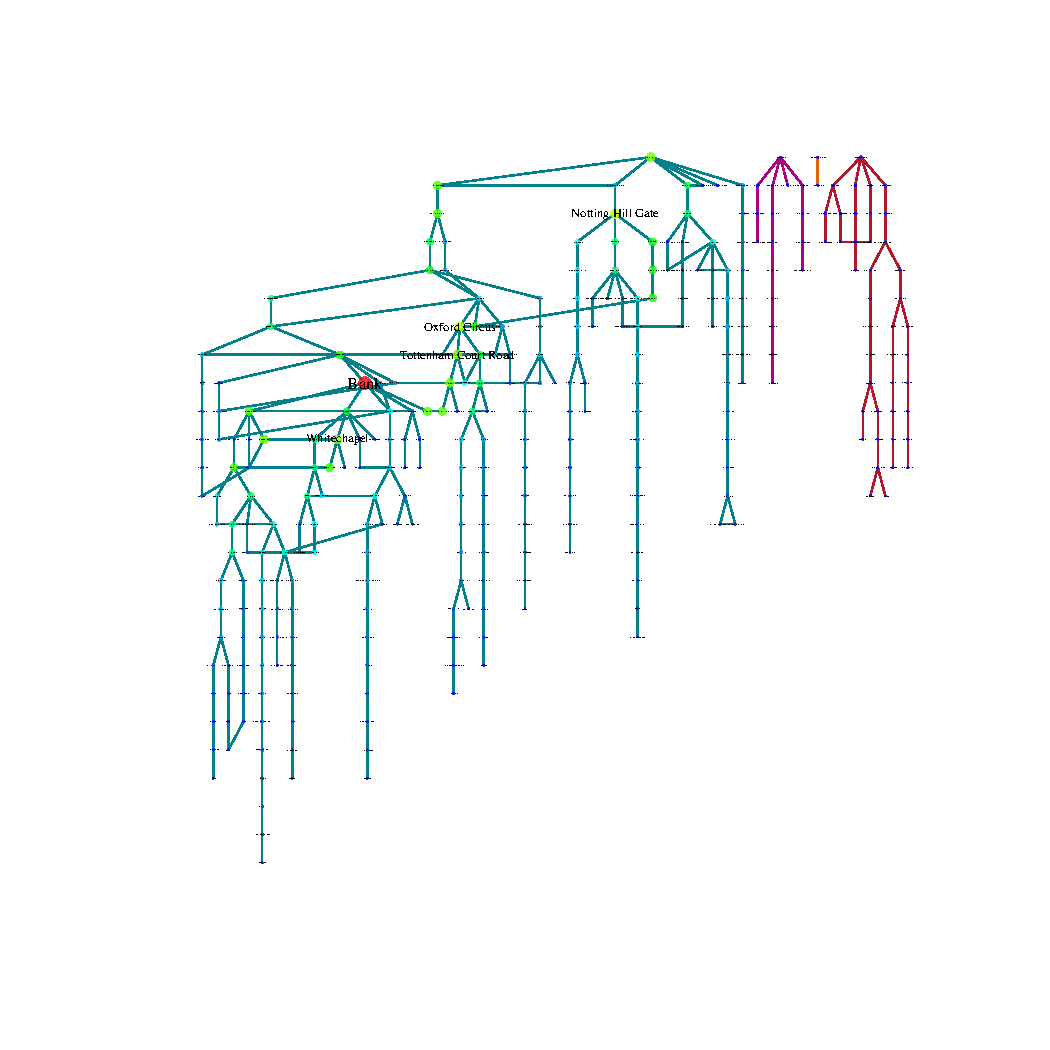
\includegraphics[clip, trim=3cm 3cm 2cm 2cm,width=1\textwidth]{images/NW/7_2.pdf}
    \caption{The tree topology of the London underground network after removing Baker Street, Ealing Common and King's Cross St. Pancras}\label{fig: 7_2}
\end{minipage}
\end{figure} 

\subsection{Final Results and Conclusion}
\label{ssec:finalresult}
\begin{table}[H]
  \centering
    \begin{tabular}{*4{c}}
    \toprule
    Romoved Nodes & \multicolumn{1}{c}{Degree} & \multicolumn{1}{c}{Betweenness} & \multicolumn{1}{c}{Eigenvector} \\
    \midrule
    King's Cross St. Pancras & 0.02431 & 0.35867 & 0.98432 \\
    King's Cross St. Pancras and Baker Street & 0.01798 & 0.34598 & 0.98471 \\
    Baker Street & 0.03085 & 0.31748 & 0.98157 \\
    Baker Street and Bank & 0.03105 & 0.31540 & 0.98498 \\
    Baker Street and Earl's Court & 0.03107 & 0.39435 & 0.98151 \\
    Baker Street  Ealing Common & 0.03101 & \cellcolor{Gray}{0.21971} & 0.98151 \\
    Baker Street  Ealing Common King's Cross St. Pancras & 0.01810 & 0.27022 & 0.98466 \\
    \bottomrule
    \end{tabular}%
    \caption{Network Centralization Scores of Each Scenario}
  \label{tab: model_result}%
\end{table}%
Table \ref{tab: model_result} shows the results of different network centrality of all the mentioned models. If we choose network betweenness centrality as the measurement of final impact,  we can see that the optimal sets of nodes that disrupts the whole system most is the combination of Baker Street and Ealing Common, which is selected based on node fragment centrality. 
\\In conclusion, based on given evidences (e.g. underground lines, topology of tube stations, distances between pairs of stations) and certain assumptions the above attack strategies were given. In the future, as more information is provided, such as the connection to other kind of transport systems and passenger flux data, these strategies would be optimized. For example, \citeauthor{jordan2008predicting} (2008) indicates that the Heathrow station would become an important target if the global air transport system is taken into consideration. 

\newpage
\section{Agent Based Models}
\label{sec:abm}
\fancyhead[R]{Agent Based Models}
\subsection{Introduction}
Agent-Based Models (ABM) and Cellular Automata Models (CA) are two commonly used urban models for complex spatial system. ABM generally simulates dynamic processes of individuals or objects while CA is based on finer spatial scales in regards to physical morphology (\cite{batty1997cellular}). Therefore, ABM is more suitable for cases containing explicit and dynamic activities or behaviors while CA deals with issues in particular related to land development, built-environment, urban growth, etc. 
\\This article aims at assessing the sensitivity of the Epidemic ABM models to varying parameter settings. This model simulates the spread of illness among a certain amount of people. Parameters like the initial population, number of infected individuals, immune chance and recovery chance are examined.
\subsection{Experiments}
\subsubsection{Change of Initial Number of Infected}
Here we set initial number of infected people to 1, 10, 50, 100, 280, respectively (see figure \ref{tab:num_infected}). It will then randomly infect this number of people if they do not have any immunity. Thus, as ticks increase, the average percentage of infected people go up (see figure \ref{fig:num_infect}). The line range represents 95\% confidence interval for each time of all repetitions. 
\\The growing trend tends to be stable afterwards. The higher initial infected number, the less time needs to reach stable infected rate level. The minimum time needed to run the simulation is around 100 times through exploratory analysis.
\\When there is only 1 infected people at the start the stable average value seems much lower than the others. However, it is due to the many cases that this infected individual recover at the first time leaving the world with no source of infection. If we ignore this phenomena, it can be conclude that under the conditions with 10\% recovery chance and 10\% immune chance, no matter how many people are initially infected (at least works for range [10:280]), the infected rate will always get stable around 45\%. Therefore, in this case, infected rate is not sensitive to the initial number of infected.
\\To find the minimum number of runs, experiments are set up with 500 repetitions and 10 number of the initial infected while other settings remain the same as before (see figure \ref{fig: run_500_avg}). The black line represents the average of additive infected rate within a certain amount of runs. The red line range indicated 95\% confidence interval.  Figure \ref{fig: rst_error} shows the corresponding standard errors after certain runs of experiments. If we set minimum standard error to 0.1 as the evidence of getting statistical meaningful results, therefore the minimum runs is supposed to be 103. However, if two of all samples are compared by Welch Two Sample t-test assuming that it's normally distributed, the mean of the results of the first two runs is significantly same (with p value equals to 0.34 $>$ 0.05) from that of the first three runs. In this case, at least two runs are required to get significant results. Similar results for more runs and the t test result p value for the comparison among 103 runs and 104 runs are around 0.9. In conclusion, the minimum runs differs as the measurement of significantly meaningful differs.

\begin{figure}[H]
\begin{minipage}[b]{0.35\linewidth}
\centering
\begin{tabular}{lr}
 	\toprule
    Parameters & \\
    \midrule
    num-infect & \multicolumn{1}{l}{1 10 50 100 280} \\
    recovery-chance & 10 \\
    initial-people & 300 \\
    immune-chance & 10 \\
    \midrule
    Repetitions & 15 \\
    Time limit & 500 \\
    \bottomrule
\end{tabular}
  \caption{Experiment Setup}
  \label{tab:num_infected}
\end{minipage}
\begin{minipage}[b]{{0.8\linewidth}}
\centering
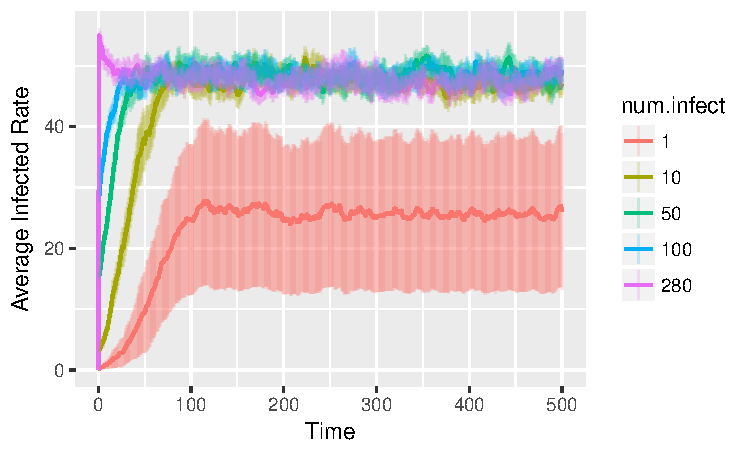
\includegraphics[{width=0.8\linewidth}]{images/ABM/num_infect.pdf}
\caption{Time vs Average Infected Rate}
\label{fig:num_infect}
\end{minipage}
\end{figure}

\begin{figure}[H]
\begin{minipage}[b]{{0.5\linewidth}}
\centering
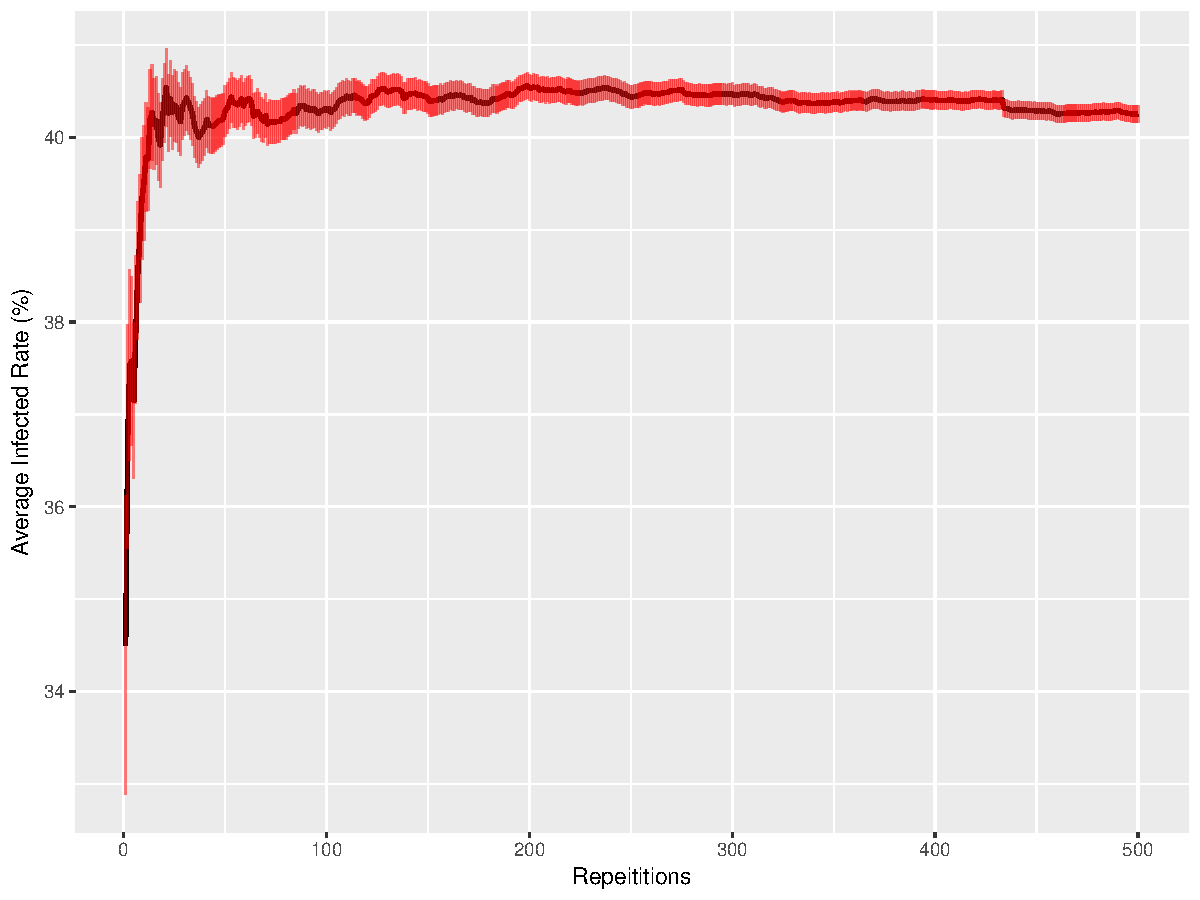
\includegraphics[{width=1\textwidth}]{images/ABM/avg.pdf}
\caption{Runs vs Average Infected Rate}
\label{fig: run_500_avg}
\end{minipage}
\begin{minipage}[b]{{0.5\linewidth}}
\centering
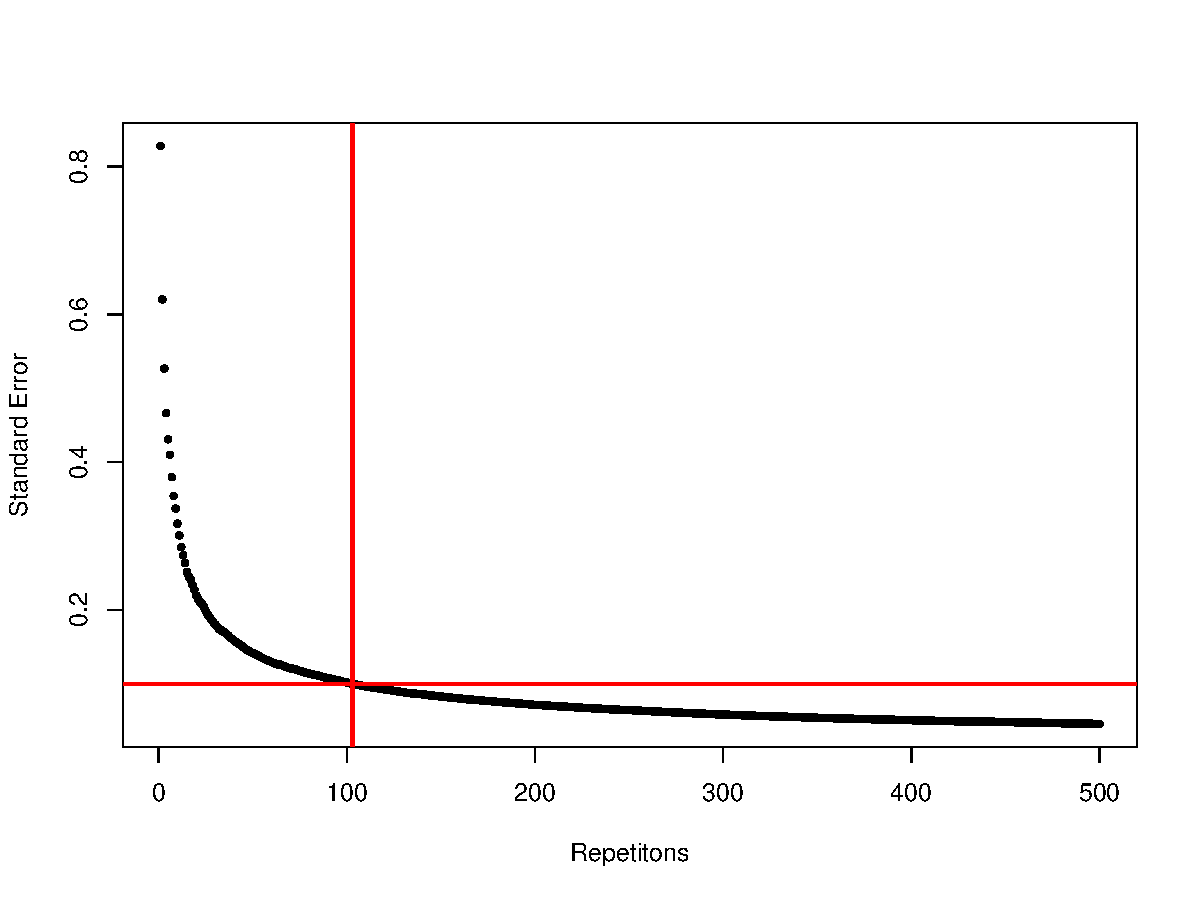
\includegraphics[{width=1\textwidth}]{images/ABM/st_error.pdf}
\caption{Runs vs Std. Error Infected Rate}
\label{fig: rst_error}
\end{minipage}
\end{figure}


\subsubsection{Multiple Parameter Settings}
By referring to the previous results, we set repetitions to 100 and time limit to 150. We change multi parameters (see figure \ref{tab:final_settings}) at the same time to see the combined effect on infected rate with extreme scenarios like 3000 population and one percent recovery rate and immune rate. From figure \ref{fig:final_plots}, it can be seen that recovery chance has much stronger effect on the change of infected rate than immune chance, which indicates that improvement on recovery chance has better efficiency on stopping the spread of diseases. In the case with 3000 initial population, what ever the changes of recover rate and immune rate are, the reached stable average infected rates are always quite high, more than 75 percent, which indicates the importance of avoiding high public population density to control diseases spread. Besides, the confidence interval of these curves is very narrow and can be hard tell in the figure.
\begin{figure}[H]
\begin{minipage}[b]{0.35\linewidth}
\centering
\begin{tabular}{lr}
 	\toprule
    Parameters & \\
    \midrule
    num-infect & 10 \\
    recovery-chance & 1 5 10 20 \\
    initial-people & 300 500 3000 \\
    immune-chance & 1 5 10 20\\
    \midrule
    Repetitions & 100 \\
    Time limit & 150 \\
    \bottomrule
\end{tabular}
  \caption{Experiment Setup}
  \label{tab:final_settings}
\end{minipage}
\begin{minipage}[b]{{0.75\linewidth}}
\centering
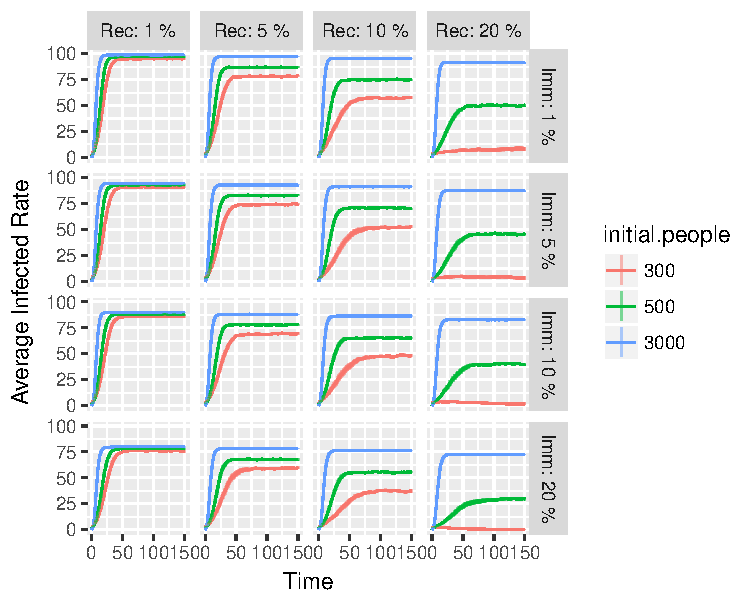
\includegraphics[width={1\textwidth}]{images/ABM/combinednew.pdf}
\caption{Multiple Parameter Settings}
\label{fig:final_plots}
\end{minipage}
\end{figure}

\subsection{Explore of Determining Minimum Runs}
In conclusion, a statistical exploratory analysis of the outcomes of ABMs especially in the form of means and standard deviations is usually necessary. Since the shape of outcomes' distribution can not be accessed previously, the time or runs at which mean and standard errors of the result reach a stable is important. However, different criteria for deciding the moment of stability suffers and falls to make a wise selection (\cite{lee2015complexities}). 
In the former subsection, we use standard error as an indicator to check the point of stability. Here, \citeauthor{lee2015complexities} introduced a scaling one which is the ratio of standard deviation of a sample ($\sigma$) to its mean ($\mu$): the coefficient of variation ($C_{v}$). 
Therefore, the method can be improved by examining the  $C_{v}$ of different sized samples. When the sample size meet the conditions that the difference between two  nearby $C_{v}$ continuously falls and under a criteria $E$ , it is considered as the minimum runs.  These $C_{v}$ stability points are contained for all interested ABM outcomes and thus the minimum number of runs is the maximum number of these $C_{v}$ points.


\newpage
\section{Spatial Interaction Models}
\label{sec:spatial}
\fancyhead[R]{Spatial Interaction Models}
First, in section \ref{ssec:spatial models}, this article briefly introduces four core members of spatial interaction models family, namely unconstrained models (subsection \ref{sssec:unconstrained models}), production constrained models (subsection \ref{sssec:production models}), attraction constrained models (subsection \ref{sssec:attraction models}) and doubly constrained model (subsection \ref{sssec:double models}). In each subsection, it starts with a brief introduction of each model's equation and assesses the role of the constraints to the model . Followed by experiments on testing the effect of varying parameters and  inputs on spatial interactions.The model is based on the commuting data among 33 boroughs in London.
\subsection{Initial Spatial Interaction Models}
\label{ssec:spatial models}
Family of spatial interaction models were initially put forward by \cite{wilson1971family}. In this article the basic gravity model is used (\cite{dennett2012estimating}, \cite{oshan2016primer} and \cite{rodrigue2016geography}).
\subsubsection{Unconstrained model}
\label{sssec:unconstrained models}
The basic unconstrained model is as follows:
\begin{equation}
T_{ij} = K O_{i} D_{j} c_{ij}^{-\beta}
\end{equation}
where K is a proportionality constant related to the rate of the event which can be calculated under the constrain that total number of trips $T$ holds unchanged overtime. Therefore, K equals to:
\begin{equation}
K=\frac{T}{\sum\limits_{ij}{O_i D_j c_{ij}^{-\beta}}}
\end{equation}
The $\beta$ relates to travel cost friction. The bigger it is, the less trips are generalised and the weaker spatial interaction of the model is. In addition, the $\alpha$ as attractiveness parameter and the $\lambda$ as emissiveness parameter are added:
\begin{equation}
T_{ij}=KO_{i}^{\lambda}D_{j}^{\alpha}c_{ij}^{-\beta}
\end{equation}
In this experiment circumstances, two attributes of origin $i$ noted as $O$ are introduced, namely origin populations and origin average salaries. Attributes of destination $j$ noted as $D$ contains destination populations and destination average salaries. Besides, cost friction $c$ is represented by distance. The only constrain is the fixed sum of all trips generated, making the model flexible to be altered by different combinations of the parameters sets to some extent. However, the drawback is that it leads to a low accuracy of the final results.
\\In order to calibrate parameters, logarithm transformation is one of the methods that make the process easier. Thus, it ends up with the following equation, and followed by poisson regression: 
\begin{equation}
\log{T}_{ij} = K + \lambda\log{O}_i+\alpha\log{D}_j-\beta\log{c}_{ij}
\end{equation}
\begin{enumerate}
\item Effects of changing K, $\beta$, $\lambda$ and $\alpha$
\\Figure \ref{fig: obs_est} shows the scatter plot of observed and estimated travel flows. It is very obvious that although these parameters change only a bit, the target increases exponentially. We examined both positive and negative value as well as 0 for $K$ value. It is found that if $K$ increases or decreases a certain value, estimated travel flows will correspondingly multiple $e$ to the power of this value times. 
\\Second, from figure \ref{fig: dis_beta} it can be seen that, the $\beta$ changes the influence of distance on spatial interactions. The higher value the $\beta$ is, the steeper decrease spatial interactions have which means the more important $\beta$ is to the change of travel flows. Figure \ref{fig: ori_pop} and \ref{fig: des_sal} show the similar positive effect of $\lambda$ and $\alpha$ on spatial interactions. The bigger they are means the more influent origin or destination attributes  are to the result. 

\begin{figure}[H]
\centering
\begin{minipage}[b]{0.49\textwidth}
\centering
    \captionsetup{width=1\linewidth}
    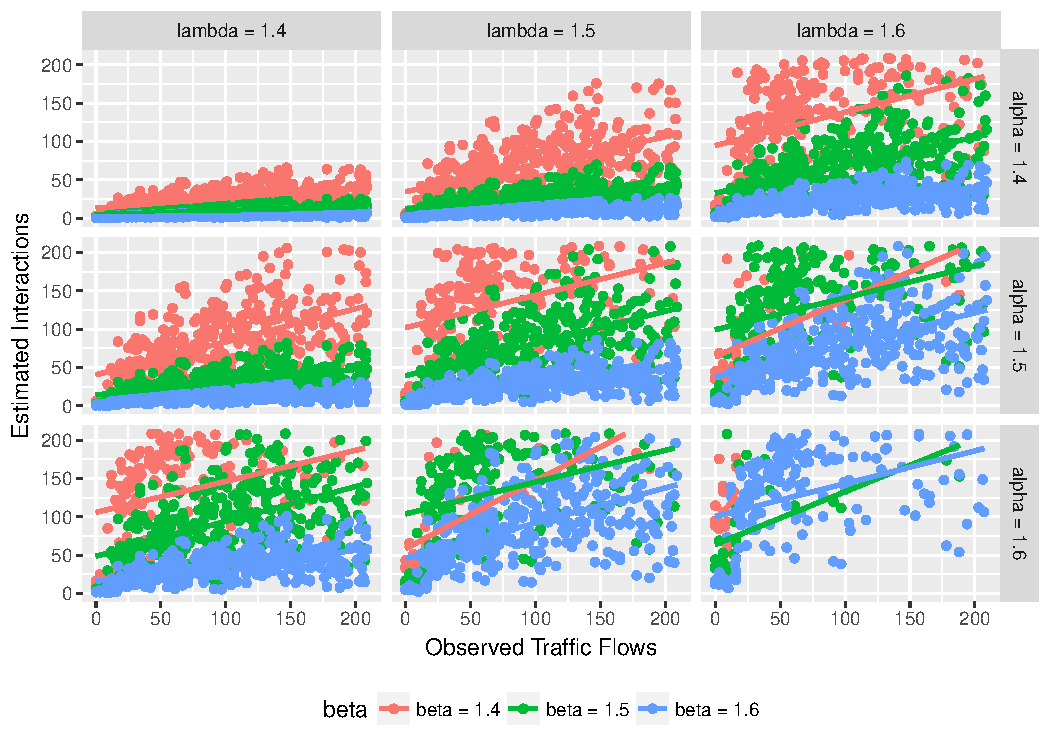
\includegraphics[width=1\textwidth]{images/SIM/obs_est.pdf}
    \caption{Observation vs Estimation}\label{fig: obs_est}
\end{minipage}
\begin{minipage}[b]{0.49\textwidth}
\centering
    \captionsetup{width=1\linewidth}
    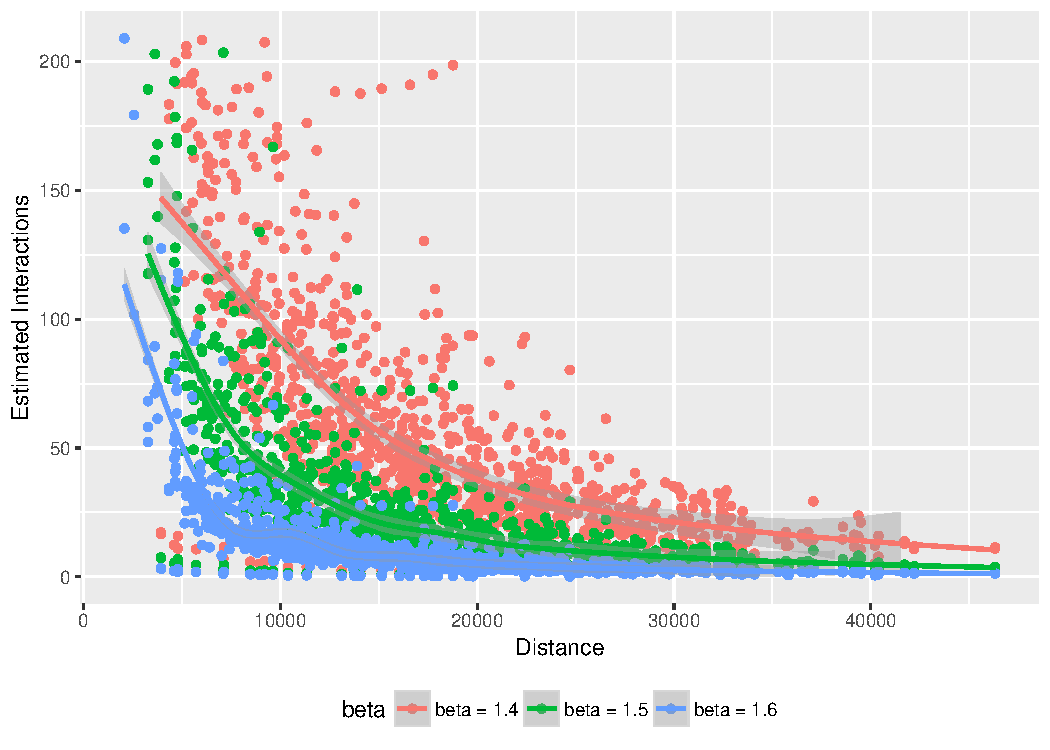
\includegraphics[width=1\textwidth]{images/SIM/dis_beta.pdf}
    \caption{Effects of $\beta$  on spatial interactions}\label{fig: dis_beta}
\end{minipage}
\end{figure} 

\begin{figure}[H]
\centering
\begin{minipage}[b]{0.49\textwidth}
\centering
    \captionsetup{width=1\linewidth}
    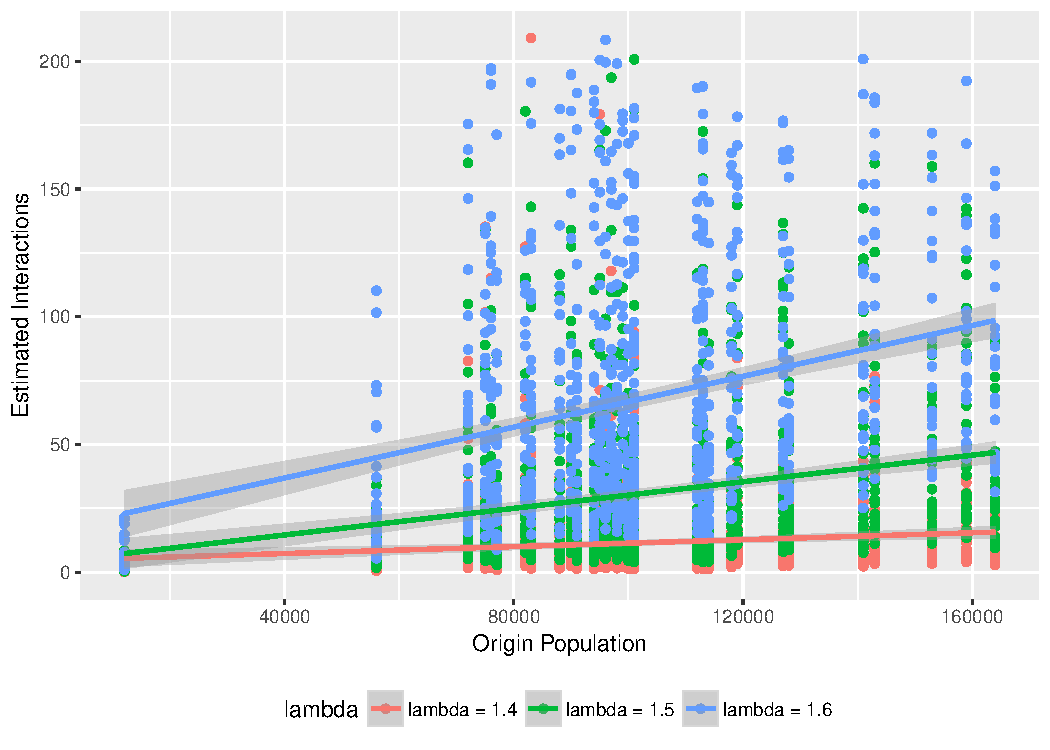
\includegraphics[width=1\textwidth]{images/SIM/ori_pop.pdf}
    \caption{Effects of $\lambda$ on spatial interactions}\label{fig: ori_pop}
\end{minipage}
\begin{minipage}[b]{0.49\textwidth}
\centering
    \captionsetup{width=1\linewidth}
    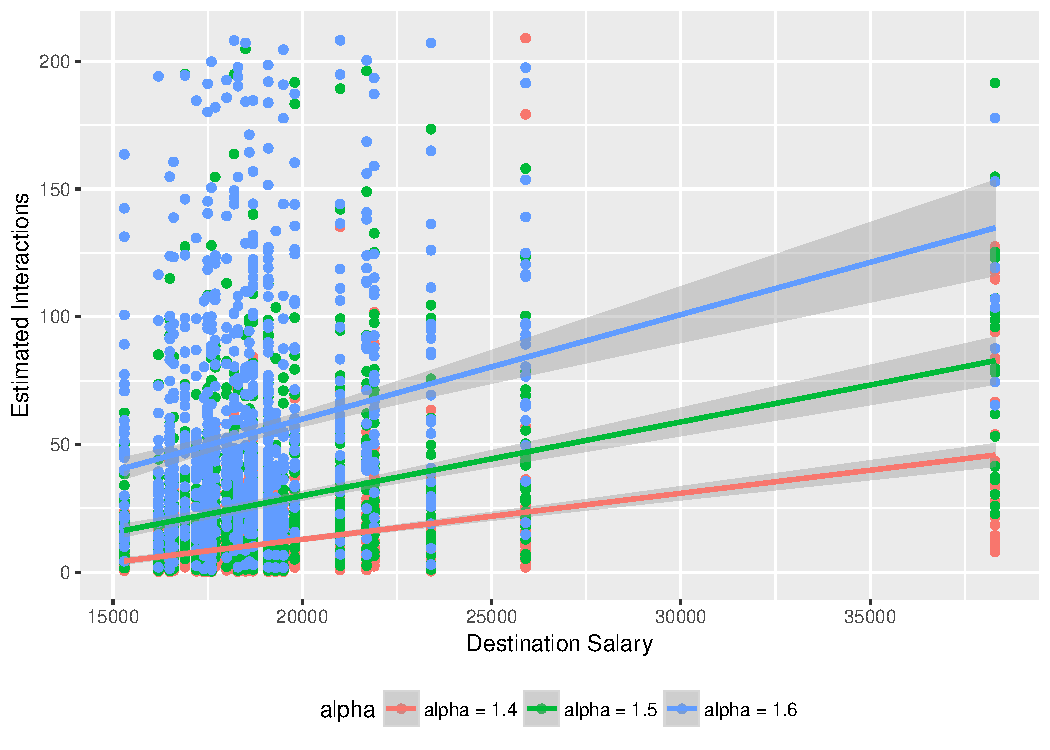
\includegraphics[width=1\textwidth]{images/SIM/des_sal.pdf}
    \caption{Effects of $\alpha$ on spatial interactions}\label{fig: des_sal}
\end{minipage}
\end{figure} 
\item Effects of Changing Inputs
\\In the case that all of a sudden a number of well paid jobs appeared in Brent and the average salary doubled, we updated the average salary data, reuse the model and calculate results again. Finally, we find that trips from boroughs to Brent all increased to around 2 times than before while other flows with increase no more than 1.15 times. From figure \ref{fig: brent} and \ref{fig: box_brent} , it can be seen that the most popular destination based on increasing flows is undoubtedly Brent while City of London, Kensington and Chelsea, and Richmond upon Thames become top three destinations with severe depopulation, which was former top three destinations with high average salary. This is all because the doubled average salary makes Brent take replace of Kensington and Chelsea becoming the second highest ranking destination.
\begin{figure}[H]
\centering
\begin{minipage}[b]{0.5\textheight}
\centering
    \captionsetup{width=1\linewidth}
    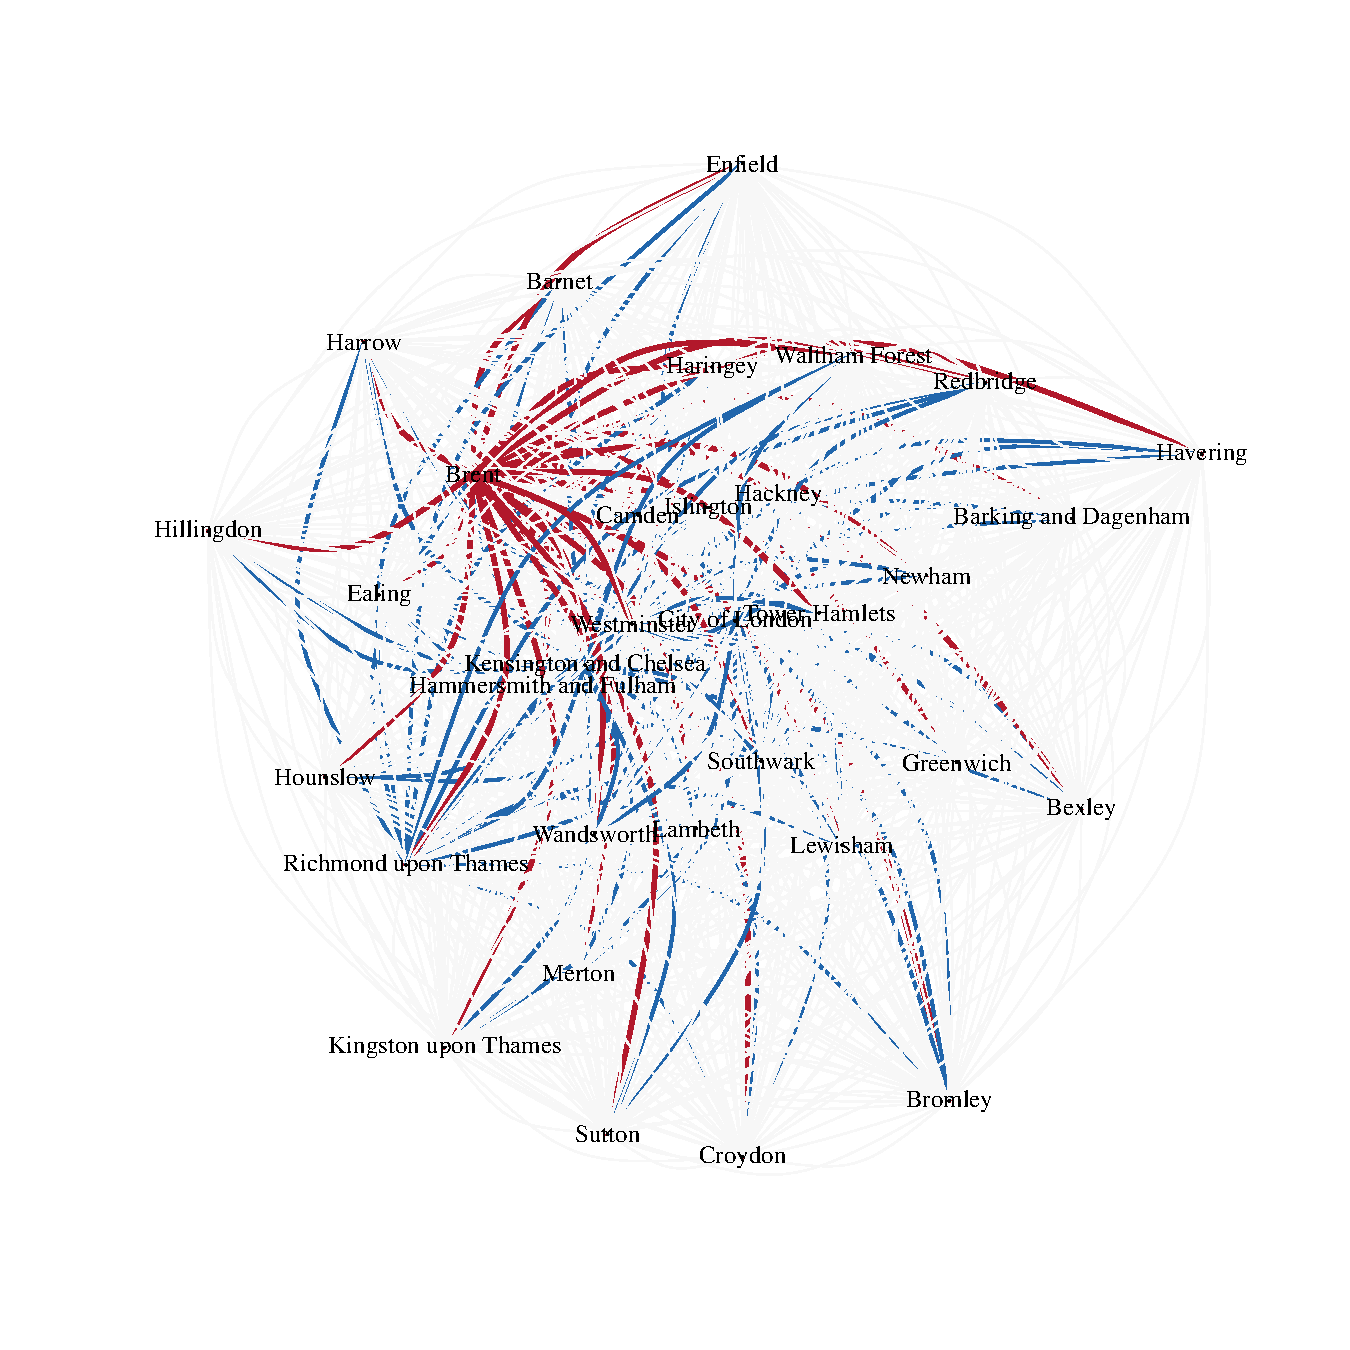
\includegraphics[clip, trim=1.5cm 3cm 2cm 2cm,width=1\textwidth]{images/SIM/Brent_final.pdf}
    \caption{Change of Travel Flows After Brent's Job Increase. Blue Line: Less Than 0.92 Times Trips Compared to Before; Red Line: More Than 2 Times Trips Compared to Before}\label{fig: brent}
\end{minipage}
\end{figure} 
\begin{figure}[H]
\centering
\begin{minipage}[b]{0.9\linewidth}
\centering
    \captionsetup{width=1\linewidth}
    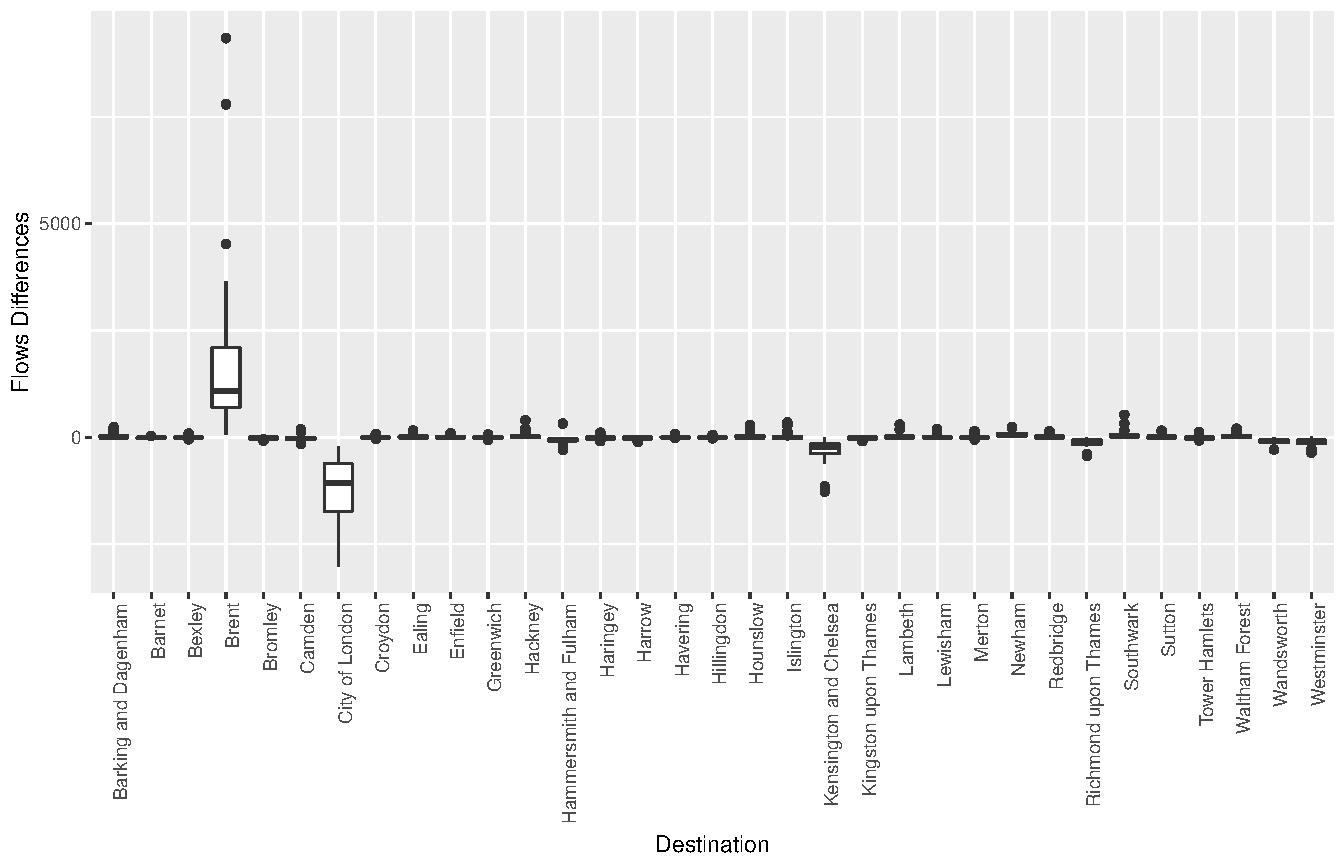
\includegraphics[clip,trim=0cm 0.2cm 0cm 3.1cm,width=1\textwidth]{images/SIM/box_brent.pdf}
    \caption{Destinations' Changes in Travel Flows After Brent's Job Increase - Unconstrained Model}\label{fig: box_brent}
\end{minipage}
\end{figure}

\end{enumerate}

\subsubsection{Production Constrained Model}
\label{sssec:production models}
In production constrained model, the total number of journeys starts within a given area, which can be stated as :
\begin{equation}
O_i=\sum_{j}T_{ij} 
\end{equation}
Thus the former model is rewritten out as:
\begin{equation}
T_{ij}=A_i O_i D_j^{\alpha} c_{ij}^{-\beta}
\end{equation}
where 
\begin{equation}
A_i=\frac{1}{\sum_{j}{D_j c_{ij}^{-\beta}}}
\end{equation}
The main difference between production constrained model and unconstrained model is that in origin constrained model, the sum of all flows for each origin is fixed. This condition to a lager extent improves the accuracy of the model. To make a comparison, we adopt the same scenario which is doubled salary in Brent to see whether there is any difference. The situation for destination estimates' change are similar as unconstrained model (see \ref{fig: box_brent}). However, for origins, the differences are clear (see figure \ref{fig: pro_orig}) with Ealing, Harrow and Barnet becoming the top three ranked origins which lose the most trips while the result for unconstrained model is not clear (see figure \ref{fig: un_orig}).
\begin{figure}[H]
\centering
\begin{minipage}[b]{1\linewidth}
\centering
    \captionsetup{width=1\linewidth}
    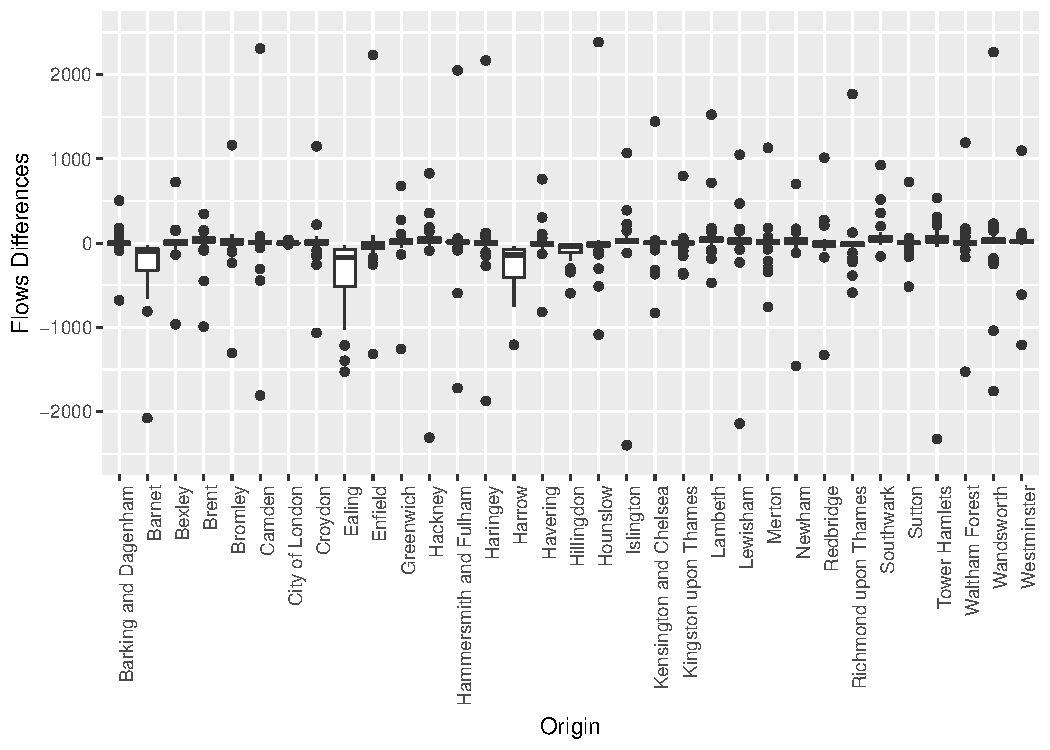
\includegraphics[width=1\textwidth]{images/SIM/pro_orig.pdf}
    \caption{Origins' Changes in Travel Flows After Brent's Job Increase - Production Constrained Model}\label{fig: pro_orig}
\end{minipage}
\end{figure} 
\begin{figure}[H]
\centering
\begin{minipage}[b]{1\linewidth}
\centering
    \captionsetup{width=1\linewidth}
    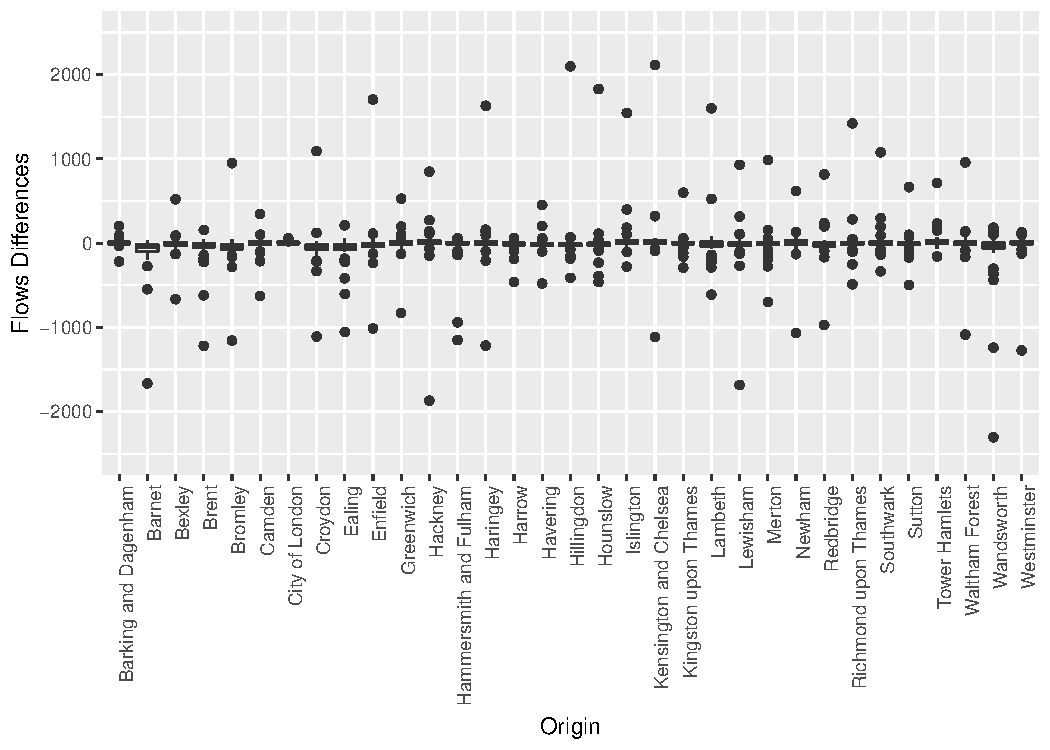
\includegraphics[width=1\textwidth]{images/SIM/un_orig.pdf}
    \caption{Origins' Changes in Travel Flows After Brent's Job Increase - Unconstrained Model}\label{fig: un_orig}
\end{minipage}
\end{figure}

\subsubsection{Attraction Constrained Model}
\label{sssec:attraction models}
In attraction constrained model, the total number of journeys ends within a given area, which can be stated as :
\begin{equation}
D_j=\sum_{i}T_{ij} 
\end{equation}
The formula is structured as :
\begin{equation}
T_{ij}=B_j D_j O_i^{\lambda} c_{ij}^{-\beta}
\end{equation}
where 
\begin{equation}
B_j=\frac{1}{\sum_{i}{O_i^{\lambda} c_{ij}^{-\beta}}}
\end{equation}
The attraction constrained model has a fixed sum of all flows for each destination. It is used under scenarios like new construction or development is finished and would attract a certain number of people to work here which indicates increase in its inbound flows. 

\subsubsection{Doubly Constrained Model}
\label{sssec:double models}
In doubly constrained model, the constrains are :
\begin{equation}
\begin{split}
O_i=\sum_{j}T_{ij}  \\
D_j=\sum_{i}T_{ij} 
\end{split}
\end{equation}
Thus the former model is rewritten out as:
\begin{equation}
T_{ij}=A_i O_i B_j D_jc_{ij}^{-\beta}
\end{equation}
where 
\begin{equation}
\begin{split}
A_i=\frac{1}{\sum_{j}{B_j D_j c_{ij}^{-\beta}}}\\
B_j=\frac{1}{\sum_{i}{A_i O_i c_{ij}^{-\beta}}}
\end{split}
\end{equation}
In this model, total numbers of both trip production and trip attraction are constrained, which makes its implementation in practicals complex and hard to process. However, it usually has the best performance among all the mentioned four models with the highest R square value and smallest RMSE value.
\subsection{Conclusion}
As \citeauthor{rodrigue2016geography} (\citeyear{rodrigue2016geography}) indicates, the process of finding a set of ideal and accurate parameters are time consuming but useful. Once a spatial interaction model for a city or region has been established, it can be used for simulation and prediction. Doubly constrained models always have the best results however it is not always easy to get reliable observed data. Therefore, single constrained models are also needed and helpful.
\newpage
\raggedright
\nocite{*}
\printbibliography
\end{document}
